\documentclass[]{book}
\usepackage[T1]{fontenc}
\usepackage{lmodern}
\usepackage{amssymb,amsmath}
\usepackage{ifxetex,ifluatex}
\usepackage{fixltx2e} % provides \textsubscript
\usepackage{booktabs}
\usepackage[export]{adjustbox}

% Added by KB to handle generation of tables with tiny font
\usepackage{floatrow}
\DeclareFloatFont{tiny}{\tiny}% "scriptsize" is defined by floatrow, "tiny" not
\floatsetup[table]{font=tiny}


\providecommand{\tightlist}{%
  \setlength{\itemsep}{0pt}\setlength{\parskip}{0pt}}

% use upquote if available, for straight quotes in verbatim environments
\IfFileExists{upquote.sty}{\usepackage{upquote}}{}
\ifnum 0\ifxetex 1\fi\ifluatex 1\fi=0 % if pdftex
  \usepackage[utf8]{inputenc}
\else % if luatex or xelatex
  \ifxetex
    \usepackage{mathspec}
    \usepackage{xltxtra,xunicode}
  \else
    \usepackage{fontspec}
  \fi
  \defaultfontfeatures{Mapping=tex-text,Scale=MatchLowercase}
  \newcommand{\euro}{€}
\fi
% use microtype if available
\IfFileExists{microtype.sty}{\usepackage{microtype}}{}
\usepackage{color}
\usepackage{fancyvrb}
\newcommand{\VerbBar}{|}
\newcommand{\VERB}{\Verb[commandchars=\\\{\}]}
\DefineVerbatimEnvironment{Highlighting}{Verbatim}{commandchars=\\\{\}}
% Add ',fontsize=\small' for more characters per line
\newenvironment{Shaded}{}{}
\newcommand{\KeywordTok}[1]{\textcolor[rgb]{0.00,0.44,0.13}{\textbf{{#1}}}}
\newcommand{\DataTypeTok}[1]{\textcolor[rgb]{0.56,0.13,0.00}{{#1}}}
\newcommand{\DecValTok}[1]{\textcolor[rgb]{0.25,0.63,0.44}{{#1}}}
\newcommand{\BaseNTok}[1]{\textcolor[rgb]{0.25,0.63,0.44}{{#1}}}
\newcommand{\FloatTok}[1]{\textcolor[rgb]{0.25,0.63,0.44}{{#1}}}
\newcommand{\ConstantTok}[1]{\textcolor[rgb]{0.53,0.00,0.00}{{#1}}}
\newcommand{\CharTok}[1]{\textcolor[rgb]{0.25,0.44,0.63}{{#1}}}
\newcommand{\SpecialCharTok}[1]{\textcolor[rgb]{0.25,0.44,0.63}{{#1}}}
\newcommand{\StringTok}[1]{\textcolor[rgb]{0.25,0.44,0.63}{{#1}}}
\newcommand{\VerbatimStringTok}[1]{\textcolor[rgb]{0.25,0.44,0.63}{{#1}}}
\newcommand{\SpecialStringTok}[1]{\textcolor[rgb]{0.73,0.40,0.53}{{#1}}}
\newcommand{\ImportTok}[1]{{#1}}
\newcommand{\CommentTok}[1]{\textcolor[rgb]{0.38,0.63,0.69}{\textit{{#1}}}}
\newcommand{\DocumentationTok}[1]{\textcolor[rgb]{0.73,0.13,0.13}{\textit{{#1}}}}
\newcommand{\AnnotationTok}[1]{\textcolor[rgb]{0.38,0.63,0.69}{\textbf{\textit{{#1}}}}}
\newcommand{\CommentVarTok}[1]{\textcolor[rgb]{0.38,0.63,0.69}{\textbf{\textit{{#1}}}}}
\newcommand{\OtherTok}[1]{\textcolor[rgb]{0.00,0.44,0.13}{{#1}}}
\newcommand{\FunctionTok}[1]{\textcolor[rgb]{0.02,0.16,0.49}{{#1}}}
\newcommand{\VariableTok}[1]{\textcolor[rgb]{0.10,0.09,0.49}{{#1}}}
\newcommand{\ControlFlowTok}[1]{\textcolor[rgb]{0.00,0.44,0.13}{\textbf{{#1}}}}
\newcommand{\OperatorTok}[1]{\textcolor[rgb]{0.40,0.40,0.40}{{#1}}}
\newcommand{\BuiltInTok}[1]{{#1}}
\newcommand{\ExtensionTok}[1]{{#1}}
\newcommand{\PreprocessorTok}[1]{\textcolor[rgb]{0.74,0.48,0.00}{{#1}}}
\newcommand{\AttributeTok}[1]{\textcolor[rgb]{0.49,0.56,0.16}{{#1}}}
\newcommand{\RegionMarkerTok}[1]{{#1}}
\newcommand{\InformationTok}[1]{\textcolor[rgb]{0.38,0.63,0.69}{\textbf{\textit{{#1}}}}}
\newcommand{\WarningTok}[1]{\textcolor[rgb]{0.38,0.63,0.69}{\textbf{\textit{{#1}}}}}
\newcommand{\AlertTok}[1]{\textcolor[rgb]{1.00,0.00,0.00}{\textbf{{#1}}}}
\newcommand{\ErrorTok}[1]{\textcolor[rgb]{1.00,0.00,0.00}{\textbf{{#1}}}}
\newcommand{\NormalTok}[1]{{#1}}
\usepackage{graphicx}
% Redefine \includegraphics so that, unless explicit options are
% given, the image width will not exceed the width of the page.
% Images get their normal width if they fit onto the page, but
% are scaled down if they would overflow the margins.
\makeatletter
\def\ScaleIfNeeded{%
  \ifdim\Gin@nat@width>.5\linewidth
    .5\linewidth
  \else
    \Gin@nat@width
  \fi
}
\makeatother
\let\Oldincludegraphics\includegraphics
{%
 \catcode`\@=11\relax%
 %\gdef\includegraphics{\@ifnextchar[{\Oldincludegraphics}{\Oldincludegraphics[width=\ScaleIfNeeded]}}%
  \gdef\includegraphics{\@ifnextchar[{\Oldincludegraphics}{\Oldincludegraphics[max size={.75\textwidth}{.75\textheight}]}}%
}%
\ifxetex
  \usepackage[setpagesize=false, % page size defined by xetex
              unicode=false, % unicode breaks when used with xetex
              xetex]{hyperref}
\else
  \usepackage[unicode=true]{hyperref}
\fi
\hypersetup{breaklinks=true,
            bookmarks=true,
            pdfauthor={Karl Benedict},
            pdftitle={Geography 485L/585L Weekly Breakdown},
            colorlinks=true,
            citecolor=blue,
            urlcolor=blue,
            linkcolor=magenta,
            pdfborder={0 0 0}}
\urlstyle{same}  % don't use monospace font for urls
\setlength{\parindent}{0pt}
\setlength{\parskip}{6pt plus 2pt minus 1pt}
\setlength{\emergencystretch}{3em}  % prevent overfull lines

\oddsidemargin = 0pt
\evensidemargin = 0pt
\topmargin = -36pt
\textwidth = 468pt
\textheight = 648pt

\setcounter{secnumdepth}{0}

\title{Geography 485L/585L Weekly Breakdown}
\author{Karl Benedict}
\date{Spring 2016}

\begin{document}
\maketitle

{
\hypersetup{linkcolor=black}
\setcounter{tocdepth}{2}
\tableofcontents
}
\chapter{Goals and Objectives}\label{goals}

Internet mapping technologies are an important component of geospatial
data capture, sharing, visualization, and delivery. This course provides
a survey of current and emerging internet and geospatial
interoperability standards, technologies, and capabilities. The emphasis
of the work in this class will be hands-on experience in four critical
aspects of Internet-enabled mapping:

\begin{itemize}
\item
  The basic concepts behind web development and web mapping technologies
  that enable the delivery of maps and mapped data through web browsers
\item
  The Open Standards that facilitate the exchange of map images and
  geospatial data over the internet
\item
  The use of published standards-based services in desktop mapping
  applications that implement those standards
\item
  The deployment of standards-based geospatial map and data services
  that other systems and users may make use of
\end{itemize}

The specific class objectives that relate to these activities and
departmental curriculum objectives for undergraduate and graduate
students in the Geography Department include the following:

\begin{itemize}
\item
  Students will understand the concepts geospatial data and service
  interoperability
\item
  Students will be able to define the specific requirements of a
  particular analysis or project and identify the interoperability
  standards that are capable of meeting those requirements
\item
  Students will be knowledgeable in the core technologies that they may
  use to produce their own internet-enabled mapping capabilities
\item
  Students will understand the strengths and limitations of current
  internet mapping technologies for generating cartographically
  effective map products.
\end{itemize}

The weekly goals, objectives and assignments are outlined below

\chapter{Week 1 - Introductions, Course Outline \& Web
Concepts}\label{week01}

This week we will review the content and structure for the course and
spend some time getting to know each other. Following this we will spend
some time setting up some of the tools that you will be using for the
course in developing your portfolio of materials.

\section{Class Prep}\label{week01-prep}

\begin{itemize}
\item
  \href{http://en.wikipedia.org/wiki/History_of_the_World_Wide_Web}{Wikipedia
  article - History of the World Wide web}
\item
  \href{http://www.lynda.com/SharedPlaylist/2b710369c9ec4d8c964467225c6610ad?org=unm.edu}{Lynda.com
  tutorials}

  \begin{itemize}
  \tightlist
  \item
    \emph{Web Design Fundamentals}

    \begin{itemize}
    \item
      Introduction
    \item
      \begin{enumerate}
      \def\labelenumi{\arabic{enumi}.}
      \tightlist
      \item
        Exploring Web Design
      \end{enumerate}
    \end{itemize}
  \item
    \emph{Version Control for Everyone}

    \begin{itemize}
    \item
      Introduction
    \item
      \begin{enumerate}
      \def\labelenumi{\arabic{enumi}.}
      \tightlist
      \item
        Introducing Version Control
      \end{enumerate}
    \item
      \begin{enumerate}
      \def\labelenumi{\arabic{enumi}.}
      \setcounter{enumi}{1}
      \tightlist
      \item
        Version Control Basics
      \end{enumerate}
    \item
      \begin{enumerate}
      \def\labelenumi{\arabic{enumi}.}
      \setcounter{enumi}{2}
      \tightlist
      \item
        Setting Up Your First Project
      \end{enumerate}
    \end{itemize}
  \end{itemize}
\end{itemize}

\section{Reference Materials}\label{week01-reference}

\href{https://github.com/UNM-GEOG-485-585/class-materials/raw/master/syllabus.pdf}{Class
Syllabus}

\section{Weekly Milestone - Creating Your GitHub Repository and First
Web Page}\label{week01-milestone}

Developing content to go onto the web has evolved from a solitary effort
to one where teams work together in developing components of larger web
sites. These teams need to have a variety of tools to enable their work.
Some of the most important tools enable code sharing with the team, and
in projects based on the \href{http://opensource.org/osd-annotated}{Open
Source} software model the rest of the world. The
\href{https://github.com/}{GitHub} web platform uses the
\href{http://git-scm.com/}{Git} distributed
\href{http://en.wikipedia.org/wiki/Revision_control}{version control}
system to enable sharing of code and hosting static web pages based on
that shared code.

You will be using a private \href{http://github.com}{GitHub} repository
to build your class portfolio during the course. If you would like to
make your portfolio available publicly you can also use GitHub as the
platform for providing that public access. Regardless of your decision
about providing public access to your portfolio, you will learn how
version control operates, and how to provide comments and keep notes on
your work and comment on the work of others (this will be part of our
peer review process).

While the work we do this and next week will be directly through the
editor integrated into the GitHub system, you will eventually need to
install a desktop application (such as the
\href{https://www.sourcetreeapp.com/}{SourceTree} application
recommended for the class) that allows you to develop your web pages on
your local computer and then update the files on the GitHub system when
you want to share a new version. Also, you can't add things like images
to your web pages until you are adding them to a local repository on
your computer and then sending them GitHub.

For this milestone we will walk through the process of creating your
repository in GitHub, creating your first web page, previewing that page
on your local computer, changing the page, and updating the page on
LoboGit. For this milestone we will do this as a manual process which we
will streamline in the coming weeks.

\emph{Step 1} - Create Your GitHub Account and Portfolio Repository

For your work in this class you will build your portfolio within an
organization (\url{https://github.com/UNM-GEOG-485-585}) within GitHub
that has been created for the class. The first step in the process of
creating your portfolio is to create a new \emph{repository} in GitHub
within which you will put your portfolio materials for sharing within
the class. Please follow the following steps to create your repository:

\begin{enumerate}
\def\labelenumi{\arabic{enumi}.}
\tightlist
\item
  Go to the \href{https://github.com/}{GitHub homepage} and follow the
  onscreen instructions for creating a new account. If you already have
  an account you can skip this step.
\item
  Come to the front of the class and tell me your GitHub username so
  that I can add you to the organization and create your repository for
  you within the organization.
\end{enumerate}

\emph{Step 2} - Create Your First Web Page

To create your first web page within your portfolio repository you need
to first enter your repository, add a new file, modify its contents, and
commit your modifications back to the repository to save your changes.

\begin{enumerate}
\def\labelenumi{\arabic{enumi}.}
\tightlist
\item
  Go to the class organization page
  ((\url{https://github.com/UNM-GEOG-485-585} - logging in if necessary)
  and click on your repository name in the list.
\item
  On the page that comes up listing the files in your repository, click
  the ``New File'' button above the list of files.
\end{enumerate}

\begin{figure}[htbp]
\centering
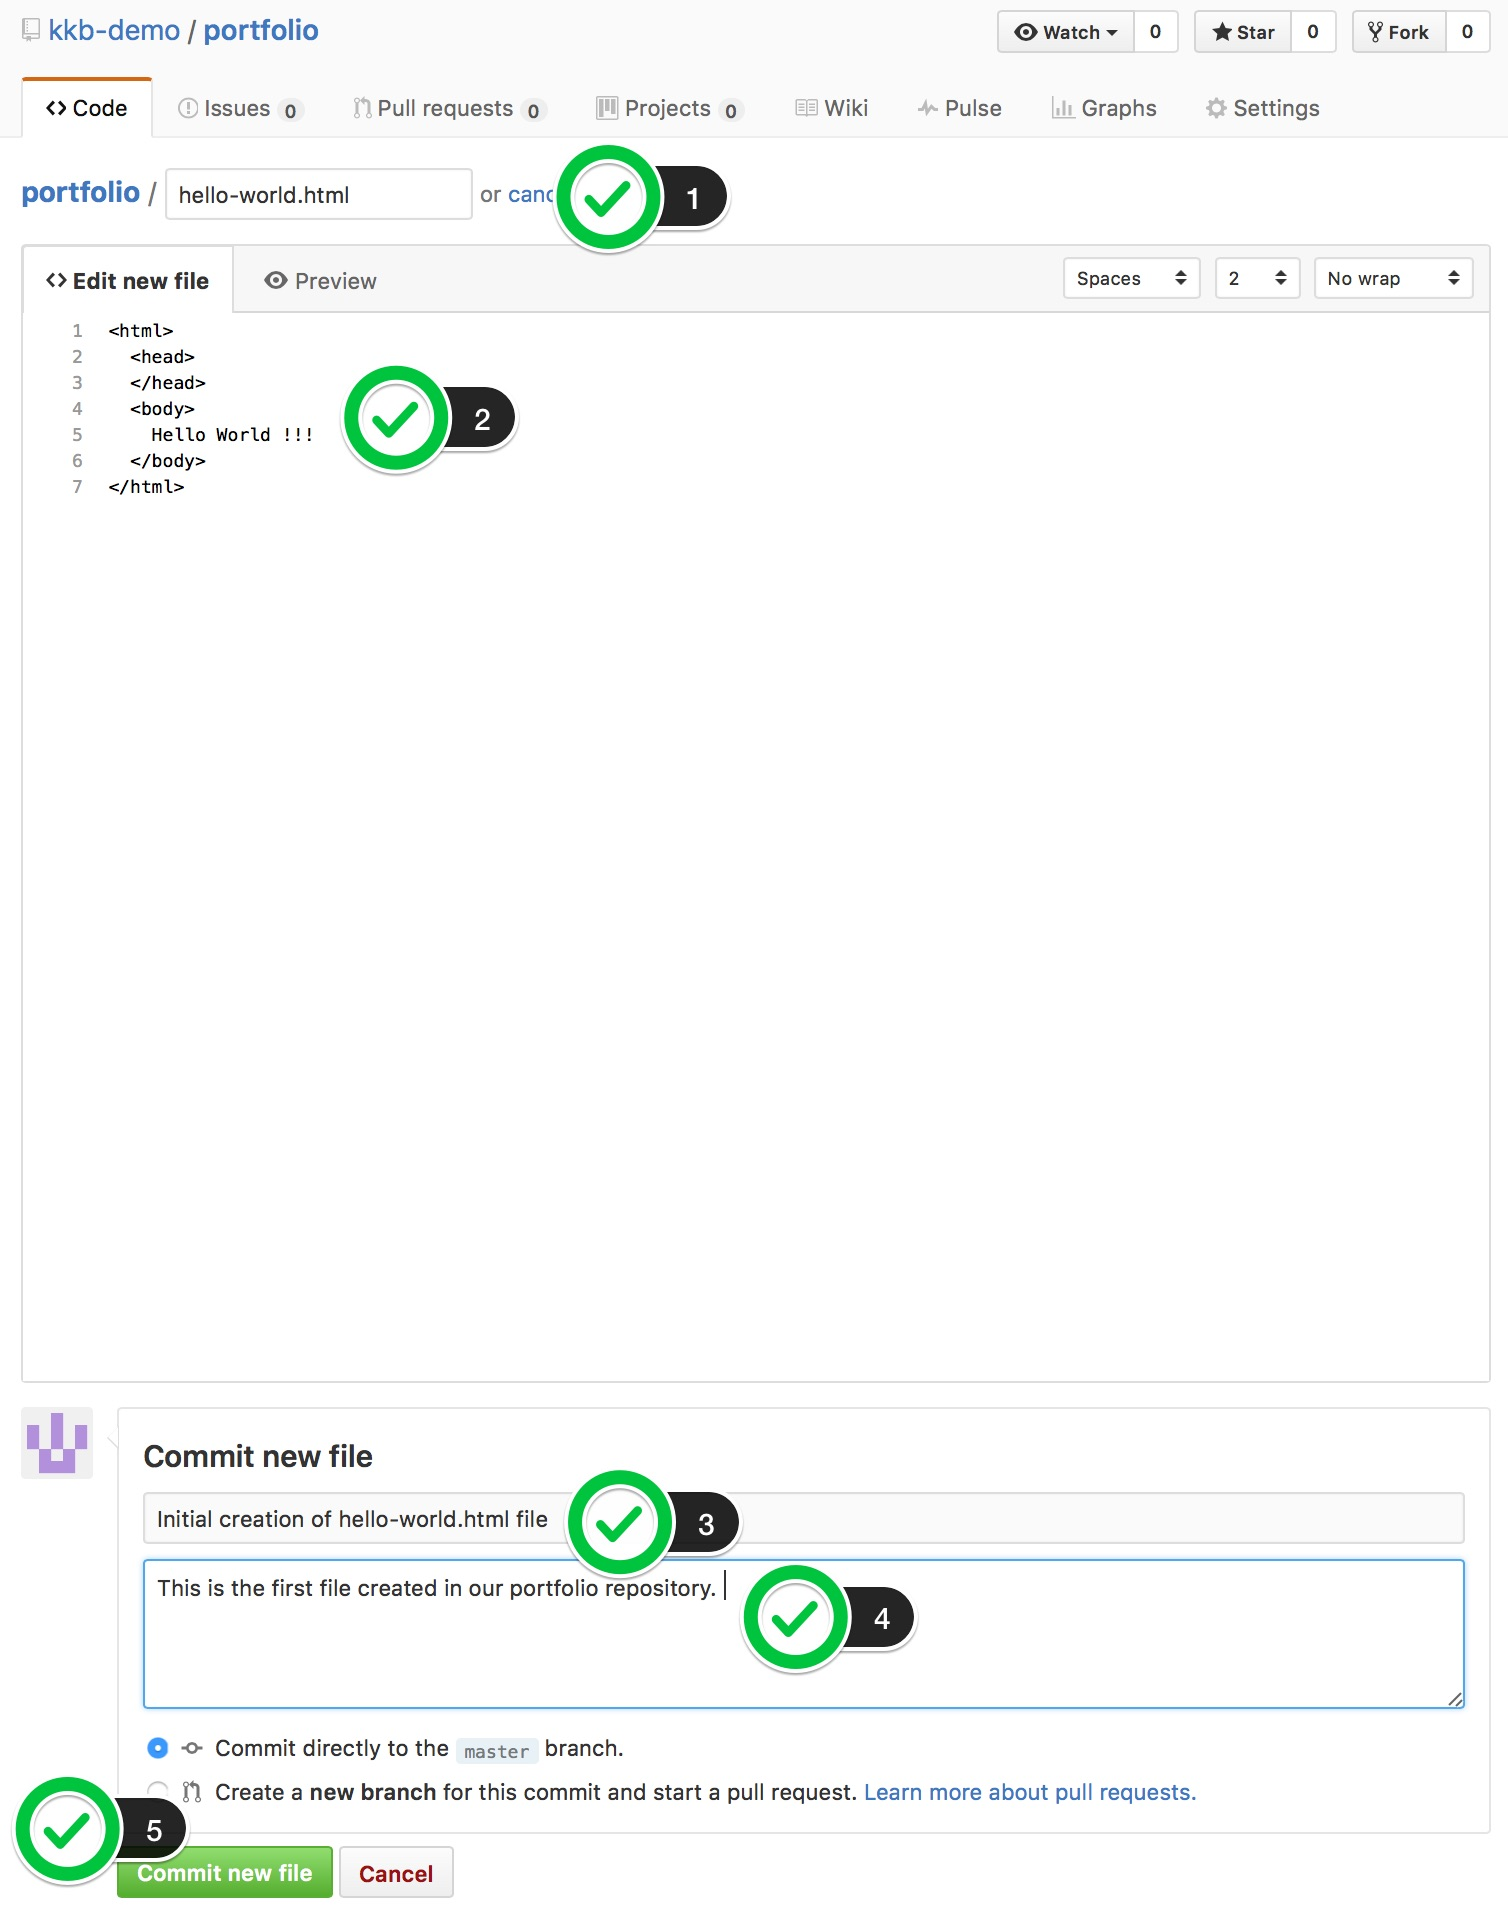
\includegraphics[width=0.70000\textwidth]{images/github_editor.png}
\caption{GitHub file creation/editor page}
\end{figure}

\begin{enumerate}
\def\labelenumi{\arabic{enumi}.}
\setcounter{enumi}{2}
\tightlist
\item
  Enter the name of the file that you are creating as
  ``hello-world.html''
\item
  Enter the following text into the text entry area under the filename
  field.
\end{enumerate}

\begin{Shaded}
\begin{Highlighting}[numbers=left,,]
\KeywordTok{<html>}
    \KeywordTok{<head>}
    \KeywordTok{</head>}     
    \KeywordTok{<body>}
        \NormalTok{Hello World !!!}
    \KeywordTok{</body>} 
\KeywordTok{</html>}
\end{Highlighting}
\end{Shaded}

\begin{enumerate}
\def\labelenumi{\arabic{enumi}.}
\setcounter{enumi}{4}
\tightlist
\item
  Add a brief comment (such as ``Created hello-world.html from provided
  text'') in the first field under the ``Commit new file'' title. You
  can optionally add a more detailed description in the next field if
  you like.
\item
  Keep the default option to ``Commit directly to the master branch''
\item
  Click the ``Commit New File'' button to commit your change and save
  the file
\end{enumerate}

\emph{Step 3} - Preview Your Web Page in a Browser

While we will later discuss strategies for hosting your web content on a
system (GitHub for example) that supports direct access by web clients,
to preview the web page you just created you need to download the
repository to your local computer where you can open the locally stored
file in a browser.

\begin{enumerate}
\def\labelenumi{\arabic{enumi}.}
\tightlist
\item
  Go to the class organization page
  ((\url{https://github.com/UNM-GEOG-485-585} - logging in if necessary)
  and click on your repository name in the list.
\item
  On the page that comes up listing the files in your repository, click
  the ``Download Zip'' button above the list of files. You may be
  prompted to provide a download location - if not you will need to find
  the default download location. Often it is the ``Downloads'' folder in
  your home directory.
\item
  Extract the contents of the downloaded .zip file using the appropriate
  utility program on your computer. On Macs and Windows computers this
  functionality is available through right-clicking on the file name in
  their respective file browsers.
\item
  Once you have extracted the contents of the zip file open the
  \texttt{hello-world.html} file that you created in a web browser -
  typically if you double-click on the file it will open in your default
  browser. You can also open it from within your browser of choice by
  using the ``Open File'' (or similar) option in the browser's file
  menu.
\item
  Confirm that the display resembles something like the following:
\end{enumerate}

\begin{figure}[htbp]
\centering
\includegraphics[width=0.70000\textwidth]{images/hello-world.png}
\caption{Sample \texttt{hello-world.html} file when viewed in a web
browser}
\end{figure}

\begin{enumerate}
\def\labelenumi{\arabic{enumi}.}
\setcounter{enumi}{5}
\tightlist
\item
  If the page does not appear as you like, edit it on GitHub and repeat
  2-5 above until you see something like the sample figure.
\end{enumerate}

\chapter{Week 2 - Module 2a - Web-based Mapping Clients: HTML, CSS \&
Javascript}\label{week02}

This week we will begin to build our foundation for developing material
to be shared over the Internet via the World Wide Web. In particular we
will cover the basic process of web development, define the parts of a
web page, and spend some time learning about the different
\emph{languages} and define the key components of a web page: its
structure, presentation, and behavior.

The presentation of information over the Internet is dependent upon the
use of standards that have been developed for defining the
\emph{structure}, \emph{presentation}, and \emph{behavior} of content.
This week we will begin working with the key technologies that define
these three components of web content.

These concepts will be illustrated through reference to several simple
web pages which are progressively modified to integrate all three of
these components.

\emph{Expected Outcomes}

By the end of this class module you should understand the following:

\begin{itemize}
\item
  The basic process of web development
\item
  The parts of a web page
\item
  The role of the three web page components: \emph{structure},
  \emph{presentation}, and \emph{behavior}
\item
  Be able to write your own basic web page with your own content and
  make it available over the web
\end{itemize}

\emph{Key Concepts}

\begin{itemize}
\item
  Parts of a web page
\item
  Structure = X/HTML
\item
  Presentation = CSS
\item
  Behavior = Javascript
\item
  Iterative Development
\end{itemize}

\section{Class Prep}\label{week02-prep}

\begin{itemize}
\item
  \href{http://www.lynda.com/SharedPlaylist/2b710369c9ec4d8c964467225c6610ad?org=unm.edu}{Lynda.com
  tutorials}

  \begin{itemize}
  \tightlist
  \item
    \emph{Web Design Fundamentals}

    \begin{itemize}
    \item
      \begin{enumerate}
      \def\labelenumi{\arabic{enumi}.}
      \setcounter{enumi}{2}
      \tightlist
      \item
        Getting Started
      \end{enumerate}
    \item
      \begin{enumerate}
      \def\labelenumi{\arabic{enumi}.}
      \setcounter{enumi}{3}
      \tightlist
      \item
        Exploring Tools
      \end{enumerate}
    \end{itemize}
  \item
    \emph{Version Control for Everyone}

    \begin{itemize}
    \item
      \begin{enumerate}
      \def\labelenumi{\arabic{enumi}.}
      \setcounter{enumi}{4}
      \tightlist
      \item
        Basic Project Sharing
      \end{enumerate}
    \item
      Conclusion
    \end{itemize}
  \end{itemize}
\item
  Duckett, Jon, and Larsen, Rob. \emph{Beginning HTML and CSS}.
  Somerset, NJ, USA: John Wiley \& Sons, 2013. ProQuest ebrary. Web. 28
  December 2015. This book is available online through the
  \href{http://site.ebrary.com.libproxy.unm.edu/lib/unma/detail.action?docID=10667426}{University
  Library} - Chapters 1, 7, 10
\end{itemize}

\section{Reference Materials}\label{week02-reference}

\begin{itemize}
\item
  Duckett, Jon, and Larsen, Rob. \emph{Beginning HTML and CSS}.
  Somerset, NJ, USA: John Wiley \& Sons, 2013. ProQuest ebrary. Web. 28
  December 2015. This book is available online through the
  \href{http://site.ebrary.com.libproxy.unm.edu/lib/unma/detail.action?docID=10667426}{University
  Library} - Chapters 2,3,4 and 8
\item
  \href{http://www.lynda.com/SharedPlaylist/2b710369c9ec4d8c964467225c6610ad?org=unm.edu}{Lynda.com
  tutorials}

  \begin{itemize}
  \tightlist
  \item
    \emph{CSS Fundamentals}
  \item
    \emph{Javascript for Web Designers}
  \end{itemize}
\end{itemize}

\section{Weekly Milestone - Create a More Complex Web Page and Style
It}\label{week02-milestone}

This week's milestone activity takes you through the process of creating
two more web pages in preparation for next week's work with the Google
Maps API in developing your first web mapping page. These pages will be:

\begin{enumerate}
\def\labelenumi{\arabic{enumi}.}
\item
  A \emph{home page} for your portfolio that will be the access point
  for all of the materials you create
  (\href{https://github.com/UNM-GEOG-485-585/class-materials/blob/master/sample-files/homePageTemplate.html}{template}/\href{http://htmlpreview.github.io/?https://github.com/UNM-GEOG-485-585/class-materials/blob/master/sample-files/homePageTemplate.html}{preview}),
  and
\item
  Your first web page containing materials related to this
  \emph{milestone} assignment
  (\href{https://github.com/UNM-GEOG-485-585/class-materials/blob/master/sample-files/assignmentTemplate.html}{template}/\href{http://htmlpreview.github.io/?https://github.com/UNM-GEOG-485-585/class-materials/blob/master/sample-files/assignmentTemplate.html}{preview}).
\end{enumerate}

\emph{Step 1} - Open the \emph{home page}
\href{https://github.com/UNM-GEOG-485-585/class-materials/blob/master/sample-files/homePageTemplate.html}{template}
linked above in your web browser and open the
\href{http://htmlpreview.github.io/?https://github.com/UNM-GEOG-485-585/class-materials/blob/master/sample-files/homePageTemplate.html}{preview}
in a second tab or window so that you can view both at the same time.

\emph{Step 2} - Copy the code in the home page
\href{https://github.com/UNM-GEOG-485-585/class-materials/blob/master/sample-files/homePageTemplate.html}{template}
into a new text file named \texttt{index.html} on your computer.

\emph{Step 3} - Open the \emph{milestone} assignment
\href{https://github.com/UNM-GEOG-485-585/class-materials/blob/master/sample-files/assignmentTemplate.html}{template}
linked above.

\emph{Step 4} - Copy the code in the template into a new text file named
\texttt{milestone\_02.html} on your copmuter.

\emph{Step 5} - After you have saved the \texttt{index.html} and
\texttt{milestone\_02.html} files to your hard drive open them up in
your browser to see what they look like when read through a web browser.

\emph{Step 6} - Add your responses to the following questions to the
\texttt{milestone\_02.html} document. - note: it is a good practice when
you are developing a web page to make small changes, save them, and
preview the page to make sure that you have not made an error in your
code before adding the next item. Practice this by adding each answer,
saving your page and previewing it and correcting any errors in your
code before going onto the next question.

\begin{description}
\item[Question 1]
From examining the display of \texttt{index.html} in your web browser
and the structure of the source code in the page, what effect (if any)
does the white space (i.e.~tabs, blank lines, multiple spaces) have on
what is displayed in the browser?
\item[Question 2]
How are the

\begin{verbatim}
<h1>
\end{verbatim}

and

\begin{verbatim}
<h2>
\end{verbatim}
\end{description}

elements from the source code displayed differently in the browser?

\begin{description}
\tightlist
\item[Question 3]
What type of element would you use to create additional list elements in
either the ``topic'' or ``data type''
(\texttt{\textless{}ul\textgreater{}}) lists on the page.
\end{description}

\emph{Step 7} - Flesh out the \texttt{index.html} page that you created
above (\emph{Step 2}) with information specific to you based upon the
content areas in the page. After making sure that your
\texttt{index.html} and \texttt{milestone\_02.html} are in the same
directory, add a \emph{relative} link to your
\texttt{milestone\_02.html} file to the ``milestones'' section of your
\texttt{index.html} page by modifying the line

\begin{verbatim}
<p><a href="">Milestone 2</a></p>
\end{verbatim}

to look like this

\begin{verbatim}
<p><a href="milestone_02.html">Milestone 2</a></p>
\end{verbatim}

Save your change and test it in the browser by clicking the link on your
\texttt{index.html} page in the browser. If it successfully opens your
\texttt{milestone\_02.html} page you have properly built your link.

\emph{Step 8} - Copy your \texttt{hello-world.html} file from
\emph{Milestone 1} into the same directory as your \texttt{index.html}
file and modify the existing line in your \texttt{index.html} file

\begin{verbatim}
<p><a href="">Hello World</a></p>
\end{verbatim}

to link to your \texttt{hello-world.html} file (follow the same pattern
you used in \emph{Step 7} above).

\emph{Step 8} - Make a copy of your \texttt{index.html} page by copying
the content of the page and pasting it into a new document named
\texttt{index\_styled.html}.

Experiment with some of the styling capabilities described in Dave
Raggett's ``Adding a Touch of Style'' page
(\url{http://www.w3.org/MarkUp/Guide/Style.html}) on
\texttt{index\_styled.html} page you created above. Make at least three
stylistic changes to the \texttt{index\_styled.html} page. Add a link to
your \texttt{index\_styled.html} page to your home page
(\texttt{index.html}) under the \texttt{milestones} section.

\emph{Step 9} - Transfer your created files \texttt{index.html},
\texttt{milestone\_02.html}, and \texttt{index\_styled.html} to your
GitHub repository (created in \emph{Milestone 1}). Of course you could
do this by copying and pasting the content of your files into
corresponding files in GitHub (but that would not be very efficient or
satisfying), but you should probably experiment with
\href{https://www.sourcetreeapp.com/}{SourceTree} as demonstrated in
this week's Lynda.com video tutorial as a way to work locally and
transfer your files to GitHub for remote access and sharing.

\chapter{Week 3 - Module 2a - Web-based Mapping Clients. Google Maps
API}\label{week03}

This week we will begin our work with the popular Google Maps
\emph{Application Programming Interface} (API) in developing an
interactive web-based mapping client. This development activity will
build upon the the work you've done over the last couple of weeks in
developing basic web pages by using the capabilities that Google has
made available for building mapping interfaces based upon their Maps
platform. You will begin working with javascript as a client programming
language to both interact with Google's servers and to provide the
needed information for Google's mapping tool in your web page.

\emph{Expected Outcomes}

By the end of this class module you should understand the following:

\begin{itemize}
\item
  What an Application Programming Interface (API) is
\item
  How Javascript can be used to define the behavior of elements in a web
  page
\item
  What the basic structure of a javascript code block for defining a
  Google Maps - enabled page looks like
\item
  How to write a basic web page that includes an interactive Google Map
\end{itemize}

\emph{Key Concepts}

\begin{itemize}
\item
  Application Programming Interface (API)
\item
  Javascript and its location within an HTML page
\item
  The interaction between javascript behaviors and structural elements
  in a web page
\end{itemize}

\section{Class Prep}\label{week03-prep}

\begin{itemize}
\item
  \href{http://www.lynda.com/SharedPlaylist/2b710369c9ec4d8c964467225c6610ad?org=unm.edu}{Lynda.com
  tutorials}

  \begin{itemize}
  \tightlist
  \item
    \emph{Javascript for Web Designers} (included as a reference source
    last week)

    \begin{itemize}
    \item
      \begin{enumerate}
      \def\labelenumi{\arabic{enumi}.}
      \setcounter{enumi}{4}
      \tightlist
      \item
        Using the Google Maps API
      \end{enumerate}
    \end{itemize}
  \end{itemize}
\item
  Svennerberg, Gabriel. \emph{Beginning Google Maps API 3}. Apress, ©
  2010. Books24x7. Web. Dec. 28, 2015.
  \href{http://library.books24x7.com.libproxy.unm.edu/toc.aspx?bookid=36390\&refid=SVA3S}{\emph{Books
  24x7 Library Database}} - if this direct link to the book doesn't work
  for you, try
  \href{http://library.unm.edu/applications/dam/plink.php?db_id=238}{logging
  in first} and searching for \texttt{Google\ Maps\ API} - the
  Svennerberg book will be the first item on the list. 1-3 (skim chapter
  2)
\end{itemize}

Continue reviewing:

\begin{itemize}
\tightlist
\item
  Duckett, Jon, and Larsen, Rob. \emph{Beginning HTML and CSS}.
  Somerset, NJ, USA: John Wiley \& Sons, 2013. ProQuest ebrary. Web. 28
  December 2015. This book is available online through the
  \href{http://site.ebrary.com.libproxy.unm.edu/lib/unma/detail.action?docID=10667426}{University
  Library} - Chapters 1, 7, 10
\end{itemize}

\section{Reference Materials}\label{week03-reference}

\begin{itemize}
\item
  Duckett, Jon, and Larsen, Rob. \emph{Beginning HTML and CSS}.
  Somerset, NJ, USA: John Wiley \& Sons, 2013. ProQuest ebrary. Web. 28
  December 2015. This book is available online through the
  \href{http://site.ebrary.com.libproxy.unm.edu/lib/unma/detail.action?docID=10667426}{University
  Library} - Chapters 2,3,4 and 8
\item
  \href{http://code.google.com/apis/maps/documentation/javascript/tutorial.html}{Google
  Maps API Tutorial}
\end{itemize}

\section{Weekly Milestone - Creation of a Web Page with an Embedded
Google Map}\label{week03-milestone}

In preparation for creating a web page with an embedded Google Map you
should first answer the following questions about what and how you want
to map. As you define the type of map you want to build, think about a
specific problem or topic that you would like to address with your map.

In this exercise you will be generating the configuration for the base
map (i.e.~The Google Maps background layers). In future assignments you
will add your own custom content to free-standing web pages that include
a mapper based upon the base map you define here.

Create a web page (based upon the assignment
\href{https://github.com/UNM-GEOG-485-585/class-materials/blob/master/sample-files/assignmentTemplate.html}{template})
that contains your milestone writeup (including the embedded Google Map
required by question 5), and link it to the home page
(\texttt{index.html}) file you created last week.

Respond to Question 1-4 with an understanding that you are generating a
web page that is designed for public viewing (even if you don't choose
to make it public at this time), and should be both clear and complete.

\begin{description}
\tightlist
\item[Question 1]
What area do you want to depict in your map? Why?
\item[Question 2]
What is the center point (latitude and longitude) of your area of
interest?
\item[Question 3]
What style of map (roads, satellite, hybrid, terrain) is appropriate for
your map? Why?
\item[Question 4]
What is the scale of your map (local, regional, continental, global)?
How will this translate into your selection of an appropriate default
zoom level for your map?
\end{description}

Now that you have answered these questions about the map that you want
to create, refer to the examples in the lecture notes, the
\href{http://code.google.com/apis/maps/documentation/javascript/tutorial.html}{Google
Maps Tutorial}, and this week's reading
(\href{https://github.com/UNM-GEOG-485-585/class-materials/tree/master/sample-files/Svennerberg_Ch3_Example}{link
to the code for Svennerberg's Chapter 3 example}) and video tutorial
assignment to create a custom Google map.

\begin{description}
\tightlist
\item[Question 5]
Embed a Google Map in your writeup that is based upon your responses to
questions 1-4 above.
\end{description}

\chapter{Week 4 - Module 2a - Web-based Mapping Clients. Google Maps
API}\label{week04}

This week covers some additional topics related to the Google Maps API,
particularly focusing on styling the Maps base maps using the
\href{http://gmaps-samples-v3.googlecode.com/svn/trunk/styledmaps/wizard/index.html}{styled
maps wizard} and integrating the javascript generated by the wizard into
the base web page code developed last week; and, using
\href{http://www.google.com/fusiontables/public/tour/index.html}{Google's
Fusion Tables} tool to create and manage tabular data for mapping and
other visualization. We complete our work with the Maps API with an
example of a more ``real'' example of a maps-enabled web page.

\emph{Expected Outcomes}

By the end of this class module you should be able to:

\begin{itemize}
\item
  Generate a Google Maps JSON style using the \emph{Styled Maps Wizard}
\item
  Integrate that JSON into your map client page for styled basemap
  display
\end{itemize}

You should also understand

\begin{itemize}
\item
  The potential of \emph{Fusion Tables} as an alternative source of data
  to integrate into a custom Google Map page
\item
  The potential structure of an \emph{operational} web page, including
  the physical separation of page components (structure, presentation,
  behavior) into separate files
\end{itemize}

\emph{Key Concepts}

\begin{itemize}
\item
  Generating Google Maps styles
\item
  Integrating styles into a Google Maps page
\item
  Fusion tables as a data source for Google Maps maps
\item
  Separation of structure, presentation, and behavior in web development
\end{itemize}

\section{Class Prep}\label{week04-prep}

\begin{itemize}
\item
  \href{http://www.lynda.com/SharedPlaylist/2b710369c9ec4d8c964467225c6610ad?org=unm.edu}{Lynda.com
  tutorials}

  \begin{itemize}
  \tightlist
  \item
    \emph{Javascript for Web Designers} (continued)

    \begin{itemize}
    \item
      \begin{enumerate}
      \def\labelenumi{\arabic{enumi}.}
      \setcounter{enumi}{4}
      \tightlist
      \item
        Using the Google Maps API
      \end{enumerate}
    \end{itemize}
  \end{itemize}
\end{itemize}

\section{Reference Materials}\label{week04-reference}

\begin{itemize}
\item
  Duckett, Jon, and Larsen, Rob. \emph{Beginning HTML and CSS}.
  Somerset, NJ, USA: John Wiley \& Sons, 2013. ProQuest ebrary. Web. 28
  December 2015. This book is available online through the
  \href{http://site.ebrary.com.libproxy.unm.edu/lib/unma/detail.action?docID=10667426}{University
  Library} - Chapters 2,3,4 and 8
\item
  \href{http://code.google.com/apis/maps/documentation/javascript/tutorial.html}{Google
  Maps API Tutorial}
\item
  \href{https://developers.google.com/maps/documentation/javascript/styling}{Google
  Maps Styling Reference}
\item
  Svennerberg, Gabriel. \emph{Beginning Google Maps API 3}. Apress, ©
  2010. Books24x7. Web. Dec. 28, 2015.
  \href{http://library.books24x7.com.libproxy.unm.edu/toc.aspx?bookid=36390\&refid=SVA3S}{\emph{Books
  24x7 Library Database}} - if this direct link to the book doesn't work
  for you, try
  \href{http://library.unm.edu/applications/dam/plink.php?db_id=238}{logging
  in first} and searching for \texttt{Google\ Maps\ API} - the
  Svennerberg book will be the first item on the list. 4-8
\item
  \href{http://earth.google.com/outreach/tutorial_fusion_yourowndata.html}{Google
  Maps Fusion Mapper}
\end{itemize}

\section{Weekly Milestone - Styling of an Embedded Google
Map}\label{week04-milestone}

Make a free-standing web page based upon the Google Map that you created
as part of last week's lab assignment. Use the Google
\href{http://gmaps-samples-v3.googlecode.com/svn/trunk/styledmaps/wizard/index.html}{styled
maps wizard} to define \emph{at least} three modified base map styles
and integrate the JSON generated by the wizard into your new Google Map
page.

\section{Deep Dive - Creation of a a Google Maps Web Page with Custom
Points and Labels}\label{week04-deepDive}

In your milestone for Week 4 you built a styled Google Maps base map for
a particular region of interest. For this \emph{deep dive} assignment
create a new free-standing web page that includes a brief description of
the topical focus of your mapper:

\begin{itemize}
\tightlist
\item
  The type of information that you want to depict in your map
\item
  Your reasons for selecting the specific area shown in the map
\item
  A description of what you are trying to communicate with the map
\end{itemize}

Embed the base map that you initially created for your milestone into
this new web page.

\begin{itemize}
\tightlist
\item
  Add 5 overlay objects to the map that relate to specific items of
  interest or importance. These overlay objects may be \emph{markers},
  \emph{polylines}, or \emph{polygons}. Make sure to include descriptive
  titles for each object.
\item
  Add an \emph{infobox} to each object that contains additional detailed
  information about the object
\end{itemize}

\chapter{Week 5 - Module 3 - GIS and Services Oriented
Architectures}\label{week05}

Core the the development of distributed mapping systems over the
internet is the concept of web services and the interoperability upon
which they are based as the means of communication between systems. This
week's lecture and focuses on the core concepts of geospatial
\emph{Services Oriented Architectures} and the open interoperability
standards from the \emph{Open Geospatial Consortium} that enable the
exchange of map images and data over the web.

\emph{Expected Outcomes}

By the end of this class module you should understand the following:

\begin{itemize}
\item
  The difference between raster and vector data formats and strategies
  for retrieving information about supported file formats
\item
  The three general tiers of a geospatial services oriented architecture
  and the components that may exist in those tiers
\item
  The key Open Geospatial Consortium standards for access, data, and
  representation
\end{itemize}

\emph{Key Concepts}

\begin{itemize}
\item
  Raster and Vector Data Models
\item
  The tiers of a geospatial services oriented architecture
\item
  The constituent components of SOA tiers
\item
  The role of OGC services in providing connectivity between SOA tiers
\item
  The OGC WMS, WFS, WCS, GML, and KML standards and their respective
  capabilities and purposes
\end{itemize}

\section{Class Prep}\label{week05-prep}

\begin{enumerate}
\def\labelenumi{\arabic{enumi}.}
\item
  Yang C, Raskin R, Goodchild M, Gahegan M. Geospatial
  Cyberinfrastructure: Past, present and future. Computers, Environment
  and Urban Systems. 2010;34: 264--277.
  doi:10.1016/j.compenvurbsys.2010.04.001
  \url{http://www.sciencedirect.com.libproxy.unm.edu/science/article/pii/S0198971510000268}
\item
  Granell C, Díaz L, Gould M. Service-oriented applications for
  environmental models: Reusable geospatial services. Environmental
  Modelling \& Software. 2010;25: 182--198.
  doi:10.1016/j.envsoft.2009.08.005
  \url{http://www.sciencedirect.com.libproxy.unm.edu/science/article/pii/S1364815209002047}
\item
  Foster I. Service-Oriented Science. Science. 2005;308: 814--817.
  doi:10.1126/science.1110411
  \url{http://science.sciencemag.org.libproxy.unm.edu/content/308/5723/814}
\end{enumerate}

\section{Reference Materials}\label{week05-reference}

None

\section{Weekly Milestone - Fun with data}\label{week05-milestone}

\begin{description}
\tightlist
\item[Question 1]
Define a data theme that you would like to focus on for this assignment
\end{description}

Download three data products from one or more of the following online
data repositories or another data repository that has data that interest
you.

\begin{itemize}
\tightlist
\item
  \href{http://rgis.unm.edu/}{New Mexico Resource Geographic Information
  System}
\item
  \href{http://nationalmap.gov/small_scale/atlasftp.html}{The US
  National Map Data Download Site}
\item
  \href{http://www.ncdc.noaa.gov/cdo-web/datasets}{NOAA's National
  Climate Data Center \emph{Climate data online: Data discovery} site}
\item
  \href{http://www.census.gov/geo/maps-data/data/tiger.html}{US Census
  Bureau - Geography - TIGER Data}
\end{itemize}

\begin{description}
\tightlist
\item[Question 2]
For each of the three datasets provide the following information
\end{description}

\begin{itemize}
\tightlist
\item
  The name of the dataset
\item
  The filename(s) for the dataset
\item
  A short (1-2 sentence) description of the dataset's contents
\item
  The bounding box (provided as the minimum and maximum extent in the
  N-S and E-W directions) in the native units and coordinate system
\item
  The coordinate reference system - by name and EPSG code
\end{itemize}

\chapter{Week 6 - Module 4.1 - Interoperability Standards - XML, KML,
and WMS}\label{week06}

This week's class focuses on three open interoperability standards that
are the most broadly used of the standards that we will be covering.

\begin{description}
\item[Extensible Markup Language (XML)]
The World Wide Web Consortium (W3C) standard that is the foundation for
many other service and data standards including: the service metadata
(GetCapabilities) for the OGC WMS, WFS, and WCS, Geography Markup
Language (GML), and KML.
\item[KML]
Formerly known as Keyhole Markup Language, an OGC standard since 2008,
KML is a combined geospatial data and representation standard that
enables the combined transfer of both location-based data and styling
information within a defined XML model.
\item[Web Map Service (WMS)]
The OGC standard for providing on-demand map visualizations based upon
user provided parameters reflecting selected data layers, defined areas
of interest, image formats, and optionally time of interest.
\end{description}

\emph{Expected Outcomes}

At the end of this class students should have an understanding of the
following:

\begin{itemize}
\item
  The basic characteristics of XML documents, including the concepts of
  \emph{well-formed} and \emph{valid} XML
\item
  The capabilities of KML for providing both data and representation
  information for geospatially referenced data.
\item
  The request-response model for OGC WMS, including the required and
  optional request parameters for the \emph{GetCapabilities},
  \emph{GetMap}, and \emph{GetFeatureInfo} requests; and the response
  types generated in response to those requests.
\item
  A general familiarity with the linkage between the WMS and KML
  standards
\end{itemize}

\emph{Key Concepts}

\begin{itemize}
\item
  XML as a general standard for structured data exchange, with DTDs and
  Schemas defining application specific data models
\item
  KML as a data and representation standard for delivery of geospatial
  data and symbolization information into client applications, both
  desktop and web-based.
\item
  WMS as a geospatial data visualization standard for providing online
  access to map images in a variety of formats for integration into
  desktop and web-based mapping applications
\end{itemize}

\section{Class Prep}\label{week06-prep}

\begin{itemize}
\tightlist
\item
  \href{http://karlbenedict.com/documents/ogcworkshop.pdf}{OGC Workshop
  White Paper}
\end{itemize}

\section{Reference Materials}\label{week06-reference}

\begin{itemize}
\item
  OGC WMS Implementation Specification
  \href{http://portal.opengeospatial.org/files/?artifact_id=7196}{Version
  1.0 - 2000},
  \href{http://portal.opengeospatial.org/files/?artifact_id=1058}{Version
  1.1 - 2001},
  \href{http://portal.opengeospatial.org/files/?artifact_id=1081\&version=1\&format=pdf}{Version
  1.1.1 - 2002},
  \href{http://portal.opengeospatial.org/files/?artifact_id=14416}{\emph{Version
  1.3.0 - 2006}}
\item
  OGC KML
  \href{http://portal.opengeospatial.org/files/?artifact_id=27810}{Version
  2.2 - 2008},
  \href{http://docs.opengeospatial.org/is/12-007r2/12-007r2.html}{\emph{Version
  2.3 - 2015}}
\item
  \href{https://developers.google.com/kml/documentation/}{Google Code
  KML Documentation}
\end{itemize}

\section{Weekly Milestone - WMS \& KML}\label{week06-milestone}

There are a large number of WMS services available on the web. One way
to find interesting services is to search for them using standard search
engines such as Google. Try searching for the following search phrase:

\texttt{“REQUEST=GetCapabilities”\ and\ “SERVICE=WMS”}

as a single search phrase

\begin{description}
\tightlist
\item[Question 1]
What search engine did you use?
\item[Question 2]
How many `hits' did you get?
\item[Question 3]
How useful (generally in terms of getting a pointers to live WMS
services {[}defined as a \emph{functioning} GetCapabilities request{]})
were the `hits'?
\end{description}

Pick two of the services that included live ``GetCapabilities'' requests
that you found above, and answer the following questions about each.

\begin{description}
\item[Question 4 (service \#1)]
What is the URL for the full GetCapabilities request to the service?

What is the Name of the service?

What Format(s) are available for GetMap requests from the service?

How many layers are included in the service (\emph{including nesting
layers})?
\item[Question 4 (service \#2)]
What is the URL for the full GetCapabilities request to the service?

What is the Name of the service?

What Format(s) are available for GetMap requests from the service?

How many layers are included in the service (\emph{including nesting
layers})?
\item[Question 5: For one of the layers in the first service,]
What is the name of the layer?

What is the SRS of the layer?

What is the name of the projection that matches the SRS EPSG code?

What is the LatLonBoundingBox of the layer?
\end{description}

Open the following GetCapabilities request in your browser. Select
``View Source'' from the browser menu to see the delivered XML document
(it may appear as an unformatted string of text by default in your
browser - if that is the case, save the file to your hard drive and view
it in a text editor). Use the information in the XML capabilities
document to formulate \texttt{GetMap} requests for the following map
images. Include the requests and resulting images in your write-up.
Comment on anything unusual that you notice in the images that are
returned.

\url{http://gstore.unm.edu/apps/rgis/datasets/92403ebf-aec5-404b-ae8a-6db41f388737/services/ogc/wms?SERVICE=wms\&REQUEST=GetCapabilities\&VERSION=1.1.1}

\begin{description}
\item[Question 6]
for the area surrounding Bernalillo County (-107.2,34.7,-106,35.25;
EPSG:4326) for the \texttt{g\_2007fe\_35\_county} layer as a 200x200
pixel JPEG

for the same area and layer as a 500x500 pixel PNG
\end{description}

Open the following (linked) KML file in Google Earth, uncompress it, and
save the contained KML file on your computer. Open the KML file in a
text editor (e.g.~Text Wrangler {[}Mac{]}, Notepad/Notepad++
{[}Windows{]}).

\url{http://rgis.unm.edu/gstore/datasets/3f0a85aa-b7f8-47bd-8db6-1c0e66becf72/nm_state_bdy_00.derived.kml}

\begin{description}
\tightlist
\item[Question 7]
Add a second \emph{Placemark} element to the KML file that represents a
\emph{square} region that is completely contained within the state
boundary. Save the KML file and open it in Google Earth (download from
http://www.google.com/earth/index.html). Submit the KML file (as a link
in your writeup) as part of your writeup for the milestone.
\end{description}

\section{Deep Dive - OGC Service Concepts}\label{week06-deepDive}

\begin{description}
\tightlist
\item[Question 1]
What request type is common across all three (WMS, WFS, WCS) OGC web
services that we have learned about?
\end{description}

Answer the following questions about a \emph{WMS GetCapabilities}
request

\begin{description}
\item[Question 2]
What are the required parameters, and what do they represent?

What is returned in response to a WMS GetCapabilities request?
\end{description}

Answer the following questions about a \emph{WMS GetMap} request

\begin{description}
\item[Question 3]
What are the required parameters, and what do they represent?

What is returned in response to a WMS GetMap request?

What is the significance of transparency in WMS requests?
\item[Question 4]
What OGC request would you use to inform the configuration of a client
application (like ArcGIS or QGIS) about an OGC service that you want to
add layers from?
\end{description}

Which OGC request would you submit under the following circumstances
(\emph{include both the service type} {[}e.g.~WMS, WFS, WCS{]}, and the
\emph{request} {[}e.g.~GetMap, GetCapabilities, GetCoverage, etc.{]} in
your answer)

\begin{description}
\item[Question 5]
You want a map image representing three layers of data in a single JPEG
for a specified area of interest.

You want to retrieve data representing geometries and associated
attributes for a road network, with the returned data in GML.

You want to retrieve data representing a digital elevation model (a
raster dataset) in the form of a GeoTIFF.
\item[Question 6 - What are the EPSG codes of the following Spatial
Reference Systems]
WGS 84 (Geodetic CRS {[}geographic 2d{]})

NAD83 / UTM zone 13N

NAD27 / UTM zone 13N
\end{description}

Retrieve the GetCapabilities XML response from the following WMS, and
answer the following questions.

\url{http://gstore.unm.edu/apps/rgis/datasets/715663ba-c1c3-414c-84a7-c671526f8316/services/ogc/wms?SERVICE=wms\&REQUEST=GetCapabilities\&VERSION=1.1.1}

\begin{description}
\item[Question 7]
What is the Title of the service?

Who is the Contact Person for questions about the service?

What are the available image formats for the GetMap request for this
service?

What are the SRS/CRS's for which layers from this service are available
(remember that nested layers inherit the SRS/CRS of their parent
layers).
\item[Question 8]
Formulate a GetMap request for the ``tl\_2010\_35\_bg10'' layer from
this service, for a 500x500 pixel map image that is 0.05-degrees wide
and 0.05-degress high, with the SW corner of the map image located at
35°N and -106°45'E (EPSG:4326). Include in your write-up the complete
GetMap request and the returned map image.
\end{description}

\chapter{Week 7 - Module 4.2 - Interoperability Standards - WFS \&
WCS}\label{week07}

This week's class focuses on two other key Open Geospatial Consortium
standards that were created to enable access to geospatial \emph{data}
of a variety of types.

\begin{description}
\item[Web Feature Service (WFS)]
A standard designed for providing on-demand access to features
(typically points, lines, and polygons and more complex combinations of
these feature types) and their associated attributes, in a variety of
formats, and optionally filtered by spatial and other query parameters.
\item[Web Coverage Services (WCS)]
A standard focused on providing access to \emph{coverages} representing
a variety of data types, but particularly optimized for dynamic delivery
of data based upon multi-dimensional gridded data.
\end{description}

\emph{Expected Outcomes}

At the end of this class students should have an understanding of the
following:

\begin{itemize}
\item
  The request-response model for OGC WFS, including the required and
  optional request parameters for the \emph{GetCapabilities},
  \emph{DescribeFeatureType}, and \emph{GetFeature} requests; and the
  response types generated in response to those requests.
\item
  The request-response model for OGC WCS, including the required and
  optional request parameters for the \emph{GetCapabilities},
  \emph{DescribeCoverage}, and \emph{GetCoverage} requests; and the
  response types generated in response to those requests.
\item
  An understanding of the distinction between WMS, WFS, and WCS for use
  in different usage scenarios (e.g.~map images, vector, raster data
  access)
\end{itemize}

\emph{Key Concepts}

\begin{itemize}
\item
  OGC WFS as a data access standard for \emph{features} and their
  attributes with support for a variety of query methods including
  spatial and parameter values.
\item
  OGC WCS as a data access standard for \emph{coverages} representing
  spatio-temporal gridded data represented in 1- or more dimensions.
\end{itemize}

\section{Class Prep}\label{week07-prep}

\section{Reference Materials}\label{week07-reference}

\begin{itemize}
\item
  {[}OGC WFS Implementation
  Specification{]}{[}http://www.opengeospatial.org/standards/wfs{]}
\item
  {[}OGC WCS Implementation
  Specification{]}{[}http://www.opengeospatial.org/standards/wcs{]}
\end{itemize}

\section{Weekly Milestone - WMS GetMap Requests, Map Scale and Aspect
Ratio Calculations}\label{week07-milestone}

You might have noticed in the WMS requests that you generated in the
previous lab returned images that didn't look ``quite right'' relative
to what you may know of the shape of familiar features.

For example, a WMS request for a 200x200 pixel PNG file (Figure
\{@fig:bernalillo-01\} for an area surrounding Bernalillo County
(-107.2,34.7,-106,35.25) from the previous lab would be
(\href{http://gstore.unm.edu/apps/rgis/datasets/92403ebf-aec5-404b-ae8a-6db41f388737/services/ogc/wms?VERSION=1.1.1\&SERVICE=WMS\&REQUEST=GetMap\&BBOX=-107.2,34.7,-106,35.25\&LAYERS=g_2007fe_35_county\&FORMAT=image/png\&TRANSPARENT=TRUE\&STYLES=\&SRS=EPSG:4326\&WIDTH=200\&HEIGHT=200}{link}):

\begin{verbatim}
http://gstore.unm.edu/apps/rgis/datasets/92403ebf-aec5-404b-ae8a-6db41f388737/
services/ogc/wms?VERSION=1.1.1&SERVICE=WMS&REQUEST=GetMap&BBOX=-107.2,34.7,
-106,35.25&LAYERS=g_2007fe_35_county&FORMAT=image/png&TRANSPARENT=TRUE&
STYLES=&SRS=EPSG:4326&WIDTH=200&HEIGHT=200
\end{verbatim}

\begin{figure}[htbp]
\centering
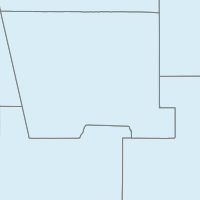
\includegraphics{images/bernalillo_01.png}
\caption{Returned map image for the region surrounding Bernalillo County
for a WMS request with \texttt{BBOX=-107.2,34.7,-106,35.25},
\texttt{WIDTH=200} and \texttt{HEIGHT=200}}
\end{figure}

this request results in a map image that does not agree with the
standard shape of Bernalillo county (depicted in QGIS - Figure
\{@fig:bernalillo-qgis\}) that we are accustomed to, regardless of the
specific map projection being used.

\begin{figure}[htbp]
\centering
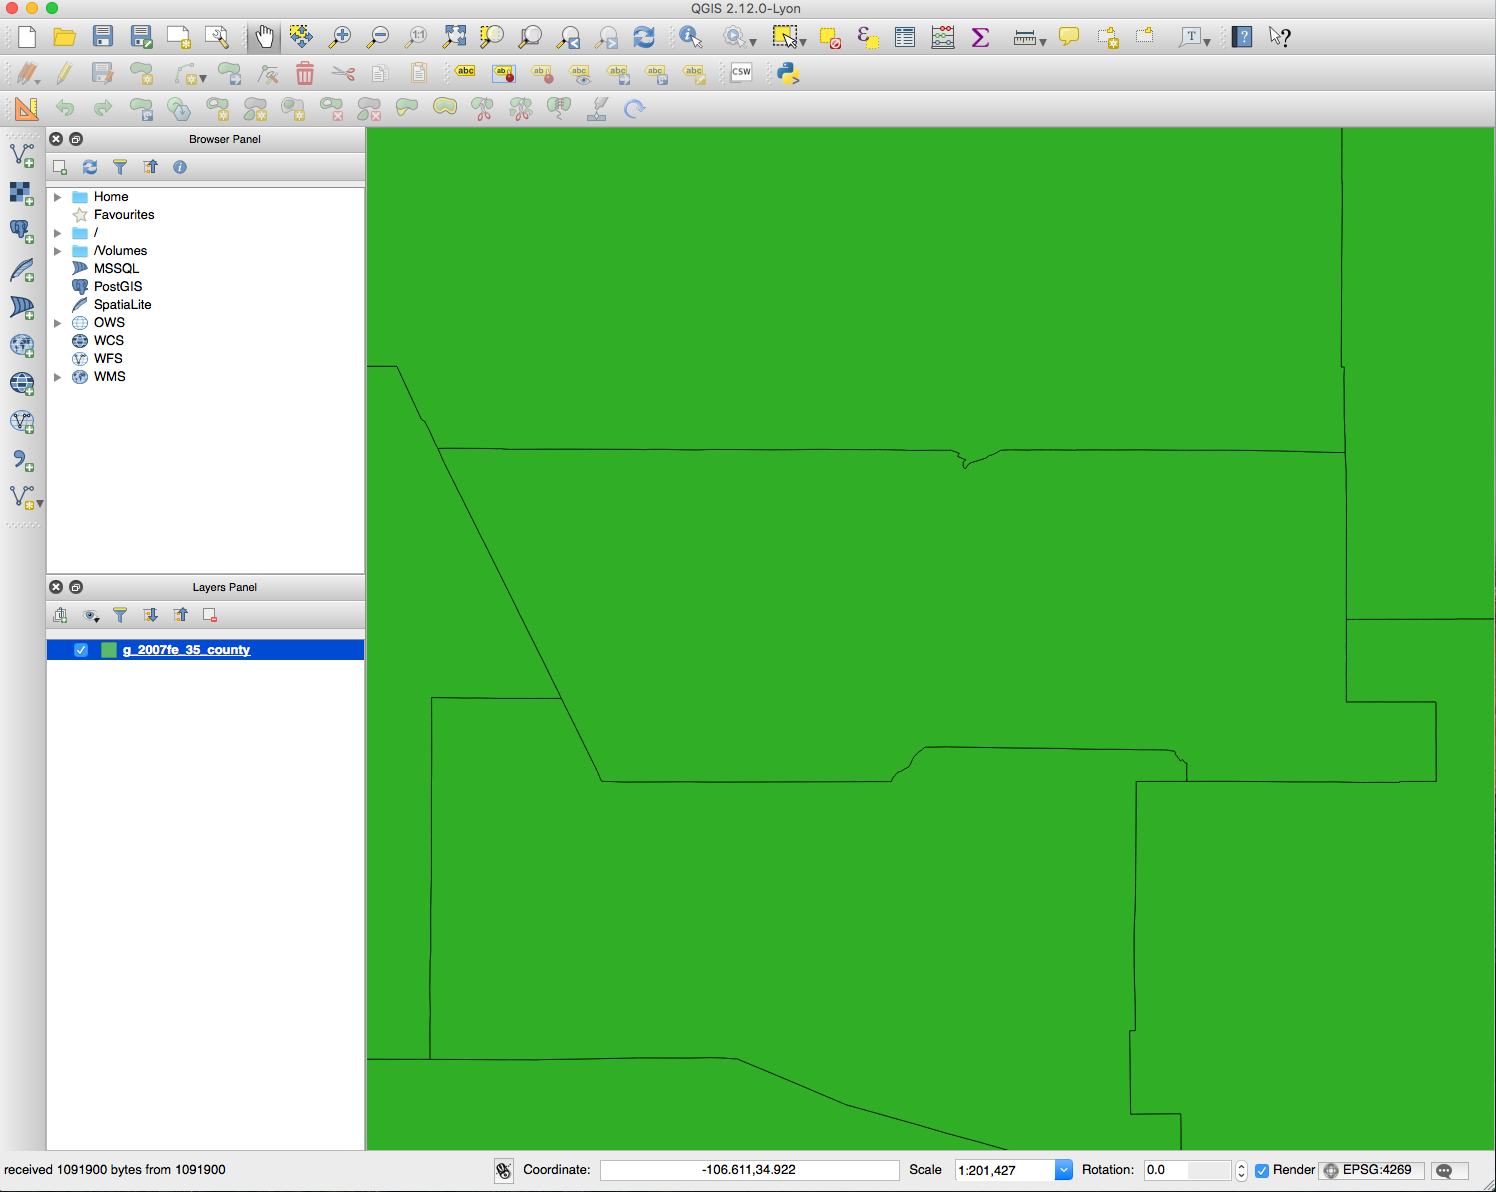
\includegraphics{images/bernalillo_qgis.png}
\caption{Area around Bernalillo County as viewed in QGIS based on the
OGC WCS based on the same data source used for the WMS request
illustrated above\}}
\end{figure}

This discrepancy is the result of a difference in the aspect ratio of
the requested BBOX (-107.2,34.7,-106,35.25) and the requested image
dimensions (200x200 pixels). \emph{When you compose a WMS GetMap
request, you need to make sure that the aspect ratio of both the image
size and BBOX match.}

For example, if we calculate the aspect ratio of the BBOX we obtain the
following values (remember that the BBOX is specified as a comma
separated list of x,y coordinates: minx,miny,maxx,maxy):

\(BBOX_{width} = x_{max} - x_{min} = (-106) - (-107.2) = 1.2^{\circ}\)

\(BBOX_{height} = y_{max} - y_{min} = 35.25 - 34.7 = 0.55^{\circ}\)

\(BBOX_{aspect-ratio} = BBOX_{width} / BBOX_{height} = 1.2^{\circ} / 0.55^{\circ} = 2.1818\)

If we want to retrieve a map image that is 200 pixels wide, we need to
calculate an image height that yields an aspect ratio that matches the
BBOX aspect ratio. Harking back to basic algebra:

\(Image_{width} = 200px\)

\(Image_{aspect-ratio} = Image_{width} / Image_{height} = 200px / Image_{height} = 2.1818\)

\(Image_{height} = Image_{width} / {aspect-ratio} = 200px / 2.1818 = 91.667px\)

So, if we request an image that is 200x92 (we have to request pixel
dimensions in integers, so rounding to the nearest integer) we should
get a representation that closely approximates the proper shape of
features. The modified WMS request with the new image's size is the
following
(\href{http://gstore.unm.edu/apps/rgis/datasets/92403ebf-aec5-404b-ae8a-6db41f388737/services/ogc/wms?VERSION=1.1.1\&SERVICE=WMS\&REQUEST=GetMap\&BBOX=-107.2,34.7,-106,35.25\&LAYERS=g_2007fe_35_county\&FORMAT=image/png\&TRANSPARENT=TRUE\&STYLES=\&SRS=EPSG:4326\&WIDTH=200\&HEIGHT=92}{link}):

\begin{verbatim}
http://gstore.unm.edu/apps/rgis/datasets/92403ebf-aec5-404b-ae8a-6db41f388737/
services/ogc/wms?VERSION=1.1.1&SERVICE=WMS&REQUEST=GetMap&BBOX=-107.2,34.7,-106,35.25&
LAYERS=g_2007fe_35_county&FORMAT=image/png&TRANSPARENT=TRUE&STYLES=&
SRS=EPSG:4326&WIDTH=200&HEIGHT=92
\end{verbatim}

\begin{figure}[htbp]
\centering
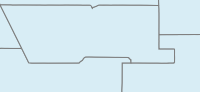
\includegraphics{images/bernalillo_02.png}
\caption{Returned map image for the region surrounding Bernalillo County
for a WMS request with \texttt{BBOX=-107.2,34.7,-106,35.25},
\texttt{WIDTH=200} and \texttt{HEIGHT=92}}
\end{figure}

This process may be reversed to request images of a fixed size for use
in a client interface, with the requested BBOX modified to match the
aspect ratio of the target image. If, for example, images are being
requested for a client interface with a fixed map size of 600x400
pixels, a corresponding BBOX can be derived using the same calculation.

If, for example, the area of interest for a map is 2 degrees wide, we
can calculate the target height (in degrees) using the aspect ratio of
the desired image.

\(Image_{aspect-ratio} = Image_{width} / Image_{height} = (600px) / (400px) = 1.5\)

\(BBOX_{aspect-ratio} = BBOX_{width} / BBOX_{height} = 2^{\circ} / BBOX_{height} = 1.5\)

\(BBOX_{height} = BBOX_{width} / BBOX_{aspect-ratio} = 2^{\circ} / 1.5 = 1.3333^{\circ}\)

If our area of interest extends from -106 to -108 degrees East
Longitude, we can use the known target height of 1.3333 to generate a
WMS BBOX of the appropriate aspect ratio. If the minimum Latitude of
interest is 34.7 degrees North Latitude, the maximum BBOX Y value would
be

\(y_{max} = y_{min} + BBOX_{height} = 34.7^{\circ} + 1.3333 = 36.0333\)

This set of calculations may be used to compose the following WMS
request
(\href{http://gstore.unm.edu/apps/rgis/datasets/92403ebf-aec5-404b-ae8a-6db41f388737/services/ogc/wms?VERSION=1.1.1\&SERVICE=WMS\&REQUEST=GetMap\&BBOX=-108,34.7,-106,36.0333\&LAYERS=g_2007fe_35_county\&FORMAT=image/png\&TRANSPARENT=TRUE\&STYLES=\&SRS=EPSG:4326\&WIDTH=600\&HEIGHT=400}{link}):

\begin{verbatim}
http://gstore.unm.edu/apps/rgis/datasets/92403ebf-aec5-404b-ae8a-6db41f388737/
services/ogc/wms?VERSION=1.1.1&SERVICE=WMS&REQUEST=GetMap&BBOX=-108,34.7,-106,36.0333&
LAYERS=2007fe_35_county&FORMAT=image/png&TRANSPARENT=TRUE&STYLES=&
SRS=EPSG:4326&WIDTH=600&HEIGHT=400
\end{verbatim}

\begin{figure}[htbp]
\centering
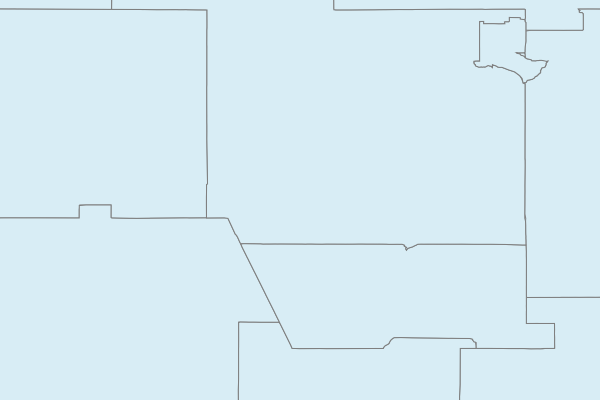
\includegraphics{images/bernalillo_03.png}
\caption{Returned map image for the region surrounding Bernalillo County
for a WMS request with \texttt{BBOX=-108,34.7,-106,36.0333},
\texttt{WIDTH=600} and \texttt{HEIGHT=400}}
\end{figure}

Given that McKinley County NM is contained within the following BBOX:
-109.5, 34.5, -106.5, 36.5

\begin{description}
\tightlist
\item[Question 1]
What is the aspect ratio (\(BBOX_{width}/BBOX_{height}\)) of this
geographic region?
\item[Question 2]
What would be the height (in whole pixels - round up) for a map image
for this region that is 600 pixels wide?
\item[Question 3]
Formulate a WMS request that reflects the values determined in 1.1 and
1.2 above for the WMS service used above in the examples and for the
\texttt{g\_2007fe\_35\_county} layer. Include in your answer both the
complete WMS request and the returned map image (either as a static
image, or an image that is linked to the live WMS).
\item[Question 4]
Formulate a WMS request for a 900x600 pixel map image that represents
the full 3-degree width of the geographic region, and is based upon the
minimum Y value of 34.5 degrees North Latitude. Include in your answer
both the WMS request and the returned map image (either as a static
image, or an image that is linked to the live WMS).
\end{description}

Given the following set of \texttt{GetMap} requests against the
\emph{\href{http://raster.nationalmap.gov/arcgis/rest/services/Orthoimagery/USGS_EROS_Ortho_SCALE/ImageServer}{USGS/EROS
Ortho Imagery Service}} answer the following questions

\begin{enumerate}
\def\labelenumi{\arabic{enumi})}
\item
  \url{http://raster.nationalmap.gov/arcgis/services/Orthoimagery/USGS_EROS_Ortho_SCALE/ImageServer/WMSServer?request=GetMap\&service=WMS\&VERSION=1.1.0\&SRS=EPSG:4326\&LAYERS=0\&FORMAT=image/jpeg\&TRANSPARENT=FALSE\&STYLES=\&WIDTH=1200\&HEIGHT=800\&BBOX=-107.1242070,34.7509960,-106.1242070,35.4176960}
\item
  \url{http://raster.nationalmap.gov/arcgis/services/Orthoimagery/USGS_EROS_Ortho_SCALE/ImageServer/WMSServer?request=GetMap\&service=WMS\&VERSION=1.1.0\&SRS=EPSG:4326\&LAYERS=0\&FORMAT=image/jpeg\&TRANSPARENT=FALSE\&STYLES=\&WIDTH=1200\&HEIGHT=800\&BBOX=-106.6867070,35.0426773,-106.5617070,35.1260148}
\item
  \url{http://raster.nationalmap.gov/arcgis/services/Orthoimagery/USGS_EROS_Ortho_SCALE/ImageServer/WMSServer?request=GetMap\&service=WMS\&VERSION=1.1.0\&SRS=EPSG:4326\&LAYERS=0\&FORMAT=image/jpeg\&TRANSPARENT=FALSE\&STYLES=\&WIDTH=1200\&HEIGHT=800\&BBOX=-106.6281133,35.0817417,-106.6203008,35.0869503}
\item
  \url{http://raster.nationalmap.gov/arcgis/services/Orthoimagery/USGS_EROS_Ortho_SCALE/ImageServer/WMSServer?request=GetMap\&service=WMS\&VERSION=1.1.0\&SRS=EPSG:4326\&LAYERS=0\&FORMAT=image/jpeg\&TRANSPARENT=FALSE\&STYLES=\&WIDTH=1200\&HEIGHT=800\&BBOX=-106.6246953,35.0840205,-106.6237187,35.0846715}
\end{enumerate}

\begin{description}
\tightlist
\item[Question 6]
Which layer(s) return map images that display image content (i.e.~return
a non-blank image)?
\item[Questions 7]
What is the difference between these requests? How might this difference
influence whether or not a map image with content is being returned?
\end{description}

\chapter{Week 10 - Web-based Mapping Clients: OpenLayers Javascript
Framework}\label{week10}

The Google Maps API provides one method for presenting an interactive
mapping tool within a web browser, but there are restrictions for free
use based upon Google's
\href{https://developers.google.com/maps/licensing}{license} agreement,
and the API is completely controlled by Google - changes are limited to
those that Google enables. The \href{http://openlayers.org/}{OpenLayers}
Javascript framework which (as quoted from the OpenLayers 2 project home
page)

\begin{quote}
has been developed to further the use of geographic information of all
kinds. OpenLayers is completely free, Open Source JavaScript, released
under the 2-clause BSD License (also known as the FreeBSD).
\end{quote}

Given its Open Source model, OpenLayers is managed as a community
software project, with the development of specific capabilities driven
by particular project or functionality needs that come out of the
community.

This week's class focuses on the basics of designing an OpenLayers
interactive mapping client, including

\begin{itemize}
\tightlist
\item
  The required structural (HTML) and behavioral (Javascript) components
\item
  Examples of creating and adding layer objects to a map
\item
  Examples of a variety of base maps that can be added to a map
\item
  The controls that may be added to a map, and the methods for managing
  and positioning those controls
\end{itemize}

\subsection{Expected Outcomes}\label{expected-outcomes}

At the end of this class the students will be able to:

\begin{itemize}
\tightlist
\item
  Create a new web page that includes an interactive OpenLayers mapper
\item
  Define one or more base map layers as part of the mapper
\item
  Define an appropriate map center and zoom level for the desired map
\item
  Enable and position controls within the map
\end{itemize}

\subsection{Key Concepts}\label{key-concepts}

At the end of this class students will understand that

\begin{itemize}
\tightlist
\item
  OpenLayers is a Javascript framework that enables web-based
  interactive mapping
\item
  The OpenLayers framework supports the integration of a variety of
  proprietary and open source base map services
\item
  Map size, center, zoom level, and layers may all be defined through
  the Javascript API
\item
  A wide variety of map controls (informational and interactive) may be
  added to maps
\end{itemize}

\section{Class Prep}\label{week10-prep}

\href{http://openlayers.org/en/v3.14.2/doc/quickstart.html}{OpenLayers
Quick Start Page}

\href{http://openlayers.org/en/v3.14.2/doc/tutorials/concepts.html}{OpenLayers
Basic Concepts}

Gratier, T., Spencer, P., \& Hazzard, E. (2015). \emph{Openlayers 3
beginner's guide : Get started with openlayers 3 and enhance your web
pages by creating and displaying dynamic maps}. Birmingham, England:
Packt Publishing.
\href{https://unm-on-worldcat-org.libproxy.unm.edu/oclc/903963849?databaseList=1271,143,1487,1533,1540,1672,1708,173,1925,2006,2007,203,2201,2237,2259,2260,2261,2262,2263,2264,2267,2268,2281,2328,3036,3201,638}{eBook}
Chapters 1-3.

\section{Reference Materials}\label{week10-reference}

\href{http://openlayers.org/en/v3.14.2/apidoc/}{OpenLayers API
Reference}

\href{http://openlayers.org/en/v3.2.1/examples/}{OpenLayers Sample Maps}

\section{Weekly Milestone - OpenLayers Mapping}\label{week10-milestone}

Following the model used in Milestone 3 for your first Google Map web
page, you should first answer the following questions about what and how
you want to map - \emph{relating to a different focus than you have used
in your previous assignments}. As you define the type of map you want to
build, think about a specific problem or topic that you would like to
address with your map.

In this exercise you will be generating the configuration for the base
map (i.e.~including one or more OpenLayer enabled background layers),
adding controls, and defining an appropriate map center and zoom level
for the map. You will add your own custom content (i.e.~the answers to
the following questions) to a free-standing web page that include an
interactive mapper and the reasoning behind the design of the map.

Create a web page that contains your milestone assignment writeup
(\emph{including} the embedded OpenLayers map required by question 5),
and link it to your home page (index.html).

Respond to Question 1-4 with an understanding that you are generating a
web page that should be clear, complete, well-formatted, and reasonably
styled.

\begin{description}
\tightlist
\item[Question 1]
What area do you want to depict in your map? Why?
\item[Question 2]
What is the center point (latitude and longitude) of your area of
interest?
\item[Question 3]
What base map(s) did you select for use in your map? Why?
\item[Question 4]
What is the scale of your map (local, regional, continental, global)?
How will this translate into your selection of an appropriate default
zoom level for your map?
\end{description}

Now that you have answered these questions about the map that you want
to create, refer to the examples in the lecture notes, the OpenLayers
Examples (\url{http://openlayers.org/en/v3.2.1/examples/}), and this
week's reading assignment to create a custom OpenLayers map.

\begin{description}
\tightlist
\item[Question 5]
Embed the OpenLayers Map in your writeup (included with the answers to
questions 1-4 above) that is based upon your responses to questions 1-4
above.
\end{description}

\section{Peer Review}\label{peer-review}

\emph{Peer Review:} This week's assignment will include a peer review
component. Specifically, 1/3 of your 20-point peer review score will be
based upon \emph{your} peer-review of \emph{two} other web pages
generated by the students in the class. The required peer-review will
consist of two steps:

\begin{enumerate}
\def\labelenumi{\arabic{enumi}.}
\item
  Create a new Discussion Thread in Learn entitled: ``Page for
  Peer-Review \textless{}Your Name\textgreater{}'' at the same time you
  link your milestone to your homepage. Include in the post the GitHub
  address of your Week 10 milestone that you created for this
  assignment.
\item
  Provide a \emph{substantive}, \emph{constructive}, and \emph{civil}
  comment (through the ``reply'' option for a posted thread) to
  \emph{two} of the posted discussion threads posted for peer-review.
  Please complete the peer-review as soon as possible so that your
  colleagues can benefit most from your input. Complete the peer-review
  no later than the required end-of-term portfolio review deadline.
  Think about the following ideas for your review: \emph{what did I
  learn from this page}, \emph{what was done well}, \emph{what could be
  improved}
\end{enumerate}

\chapter{Week 11 - OpenLayers Javascript Framework}\label{week11}

\emph{Background}

As we learned in our introduction to OpenLayers in last week's class, it
provides a flexible platform for integrating geospatial data from a
variety of sources in a single interactive mapping environment. These
capabilities include data integration from OGC Web Map Services and a
wide variety of data formats for display in the mapper. This week's
class provides an overview of the options for the OpenLayers
\texttt{Map} and \texttt{Layer} objects, and specific information about
configuring OGC WMS, KML, and Vector Geometry Layers and a brief
overview of styling of vector data layers.

\emph{Expected Outcomes}

At the end of this class, students should be able to:

\begin{itemize}
\tightlist
\item
  Create a new map object
\item
  Add a WMS layer to that map
\item
  Add a KML layer to that map
\item
  Add a variety of Vector Geometry objects to the map
\item
  Define styles for the created KML and Vector Feature objects.
\end{itemize}

\emph{Key Concepts }

At the end of this class students will understand that

\begin{itemize}
\tightlist
\item
  There are a wide variety of options that may be provided when creating
  \texttt{Map} Nd \texttt{Layer} objects within OpenLayers
\item
  WMS layers may be added to a map from diverse online servers
\item
  KML files may be added to map, but their potential size can pose a
  challenge to effective integration into online mapping applications
\item
  A wide variety of geometric objects may be defined and added to a map
\item
  There exist a variety of styling options for vector data that are
  added to a map
\end{itemize}

\section{Class Prep}\label{week11-prep}

Gratier, T., Spencer, P., \& Hazzard, E. (2015). \emph{Openlayers 3
beginner's guide : Get started with openlayers 3 and enhance your web
pages by creating and displaying dynamic maps}. Birmingham, England:
Packt Publishing.
\href{https://unm-on-worldcat-org.libproxy.unm.edu/oclc/903963849?databaseList=1271,143,1487,1533,1540,1672,1708,173,1925,2006,2007,203,2201,2237,2259,2260,2261,2262,2263,2264,2267,2268,2281,2328,3036,3201,638}{eBook}
Chapters 4-6.

OpenLayers 3 Examples:

\begin{itemize}
\tightlist
\item
  \href{http://openlayers.org/en/v3.2.1/examples/wms-image.html?q=wms}{\emph{Single
  Image WMS Example}}
\item
  \href{http://openlayers.org/en/v3.2.1/examples/wms-tiled.html?q=wms}{\emph{Tiled
  WMS Exmaple}}
\item
  \href{http://openlayers.org/en/v3.2.1/examples/icon.js}{\emph{Vector
  Icon Example}}
\end{itemize}

\section{Reference Materials}\label{week11-reference}

\href{http://openlayers.org/en/v3.14.2/apidoc/}{OpenLayers API
Reference}

\href{http://openlayers.org/en/v3.2.1/examples/}{OpenLayers Sample Maps}

\section{Weekly Milestone - A Customized OpenLayers Mapping
Client}\label{week11-milestone}

Please create a new OpenLayers mapping page that is based upon the
initial map (and thematic focus) that you created for last week's
milestone, and add the following to your map:

\begin{enumerate}
\def\labelenumi{\arabic{enumi}.}
\item
  Five Vector Features (based upon Point, LineString, or LinearRing
  Geometries), each assigned its own style.
\item
  One KML Layer, also styled. Make sure to give some thought to the size
  of the KML file that you use as large KML files can cause slow page
  loads and can in some cases crash your browser.
\item
  One WMS Layer.
\end{enumerate}

\section{Deep Dive -}\label{week11-deepDive}

This deep dive is the first of two (plus milestones) that are related to
a common theme of taking an online mapping problem from start to finish
- from the definition of a problem, through the implementation of
services and a basic client interface for the display of data for the
specific problem.

Before beginning to work on any mapping problem (online or otherwise),
some basic questions need to asked and answered. Please consider and
answer (in 2-4 sentences as appropriate for the question) the following
questions relating to the problem that you will be working on for the
forthcoming assignments:

\begin{itemize}
\item
  What is the high-level description of the problem/question you want to
  help answer through the presentation of a collection of geographic
  data over the internet? Please answer in a short paragraph.
\item
  Who is the target audience for the information you want to provide?
\item
  What geographic region does your problem area represent? Please
  describe it in words (e.g.~New Mexico, Alberta Canada, etc.) and
  define it in terms of a geographic (WGS84) (latitude and longitude)
  bounding box.
\item
  What types of data do you want to include in your project? Include a
  description (data content: e.g.~elevation data, hydrographic survey,
  etc.) and types (i.e.~raster, vector).
\item
  What projection will you use for the presentation of your project
  data? Again, describe it, provide your reasoning for selection, and
  provide the corresponding EPSG code.
\item
  Where do you anticipate acquiring data for the project from?
\item
  What barriers to acquiring and processing the needed data do you
  anticipate?
\end{itemize}

While you are going to continue to acquire additional data for the
project over the next couple of assignments, begin acquiring data for
your selected project now. Specifically, find 5 datasets that are
consistent with your description of the problem you are going to work
on, and use your desktop GIS and any associated metadata to describe
them in brief by answering the following questions:

\begin{itemize}
\item
  What is the name of the dataset?
\item
  What type of data (raster/vector) are in the dataset?
\item
  What is its format?
\item
  What is its coordinate reference system?
\item
  What are the spatial extents of the dataset?
\end{itemize}

For a dataset to be useful, you should be able to answer all five of
these questions about it. Furthermore, you should seek out datasets that
are in common formats that you know you can work with in a variety of
applications (i.e.~QGIS, ArcGIS, gdalinfo, ogrinfo, etc.). If you can't
access and use a dataset in one of these applications, you will probably
have problems trying to use it in your project.

Also, below are links to the documentation for GeoServer - the platform
that we will work with in a couple of weeks for publishing data -
relating to the supported raster and vector formats in the default
GeoServer installation.

Vector Data:
\url{http://docs.geoserver.org/stable/en/user/data/vector/index.html}

Raster Data
\url{http://docs.geoserver.org/stable/en/user/data/raster/index.html}

\section{Peer Review}\label{peer-review-1}

\emph{Peer Review:} This week's assignment will include a peer review
component. Specifically, 1/3 of your 20-point peer review score will be
based upon \emph{your} peer-review of \emph{two} other web pages
generated by the students in the class. The required peer-review will
consist of two steps:

\begin{enumerate}
\def\labelenumi{\arabic{enumi}.}
\item
  Create a new Discussion Thread in Learn entitled: ``Page for
  Peer-Review \textless{}Your Name\textgreater{}'' at the same time you
  link your milestone to your homepage. Include in the post the GitHub
  address of your Week 10 milestone that you created for this
  assignment.
\item
  Provide a \emph{substantive}, \emph{constructive}, and \emph{civil}
  comment (through the ``reply'' option for a posted thread) to
  \emph{two} of the posted discussion threads posted for peer-review.
  Please complete the peer-review as soon as possible so that your
  colleagues can benefit most from your input. Complete the peer-review
  no later than the required end-of-term portfolio review deadline.
  Think about the following ideas for your review: \emph{what did I
  learn from this page}, \emph{what was done well}, \emph{what could be
  improved}
\end{enumerate}

\chapter{Week 12 - Module 4.3 - Interoperability Standards - Desktop GIS
Integration}\label{week12}

As we've discussed the components of the client tier of our tiered
geospatial services oriented architecture we have concentrated on the
open standards that can support client applications and the web-based
clients that can consume them. Desktop GIS applications can also consume
standards-based services, specifically OGC services. This week's class
concentrates on the methods for integrating OGC services into two GIS
client applications Quantum GIS and ArcGIS, demonstrating the utility of
using external standards-based services as a data and map image source
within desktop applications.

\emph{Expected Outcomes}

At the end of this class, students should be able to:

\begin{itemize}
\tightlist
\item
  Add a WMS service to Quantum GIS
\item
  Add a WFS service to Quantum GIS
\item
  Add WMS, WFS, and WCS services to ArcGIS (if they have access to the
  required software)
\end{itemize}

\emph{Key Concepts}

At the end of this class students will understand that

\begin{itemize}
\tightlist
\item
  The key to configuring a desktop client application is the
  GetCapabilities request for the needed service
\item
  The GetCapabilities request required by a particular client may
  consist of a base URL or a complete URL.
\item
  Quantum GIS uses a base URL request model for self-configuration of
  WMS and WFS services
\item
  ArcGIS uses a base URL request model for self-configuration of WMS,
  WCS, and WFS services
\item
  Both Quantum GIS and ArcGIS require additional configuration to enable
  WFS access
\end{itemize}

\section{Class Prep}\label{week12-prep}

\begin{itemize}
\tightlist
\item
  Quantum GIS
  \href{http://docs.qgis.org/2.8/en/docs/user_manual/}{documentation},
  especially

  \begin{itemize}
  \tightlist
  \item
    \href{http://docs.qgis.org/2.8/en/docs/user_manual/working_with_ogc/index.html}{Working
    with OGC Data}
  \end{itemize}
\item
  ArcGIS \href{}{}, especially

  \begin{itemize}
  \tightlist
  \item
    \href{http://desktop.arcgis.com/en/arcmap/10.3/map/web-maps-and-services/about-using-ogc-service-layers.htm}{About
    using OGC service layers}
  \item
    \href{http://desktop.arcgis.com/en/arcmap/10.3/manage-data/using-arccatalog/connecting-to-gis-servers.htm}{Connecting
    to GIS servers}
  \item
    \href{http://desktop.arcgis.com/en/arcmap/10.3/map/web-maps-and-services/adding-wms-services.htm}{Adding
    WMS services}
  \item
    \href{http://desktop.arcgis.com/en/arcmap/10.3/map/web-maps-and-services/adding-a-wcs-service-to-arcmap.htm}{Adding
    a WCS service to ArcMap}
  \item
    \href{http://desktop.arcgis.com/en/arcmap/10.3/map/web-maps-and-services/adding-a-wfs-service-to-arcmap.htm}{Adding
    a WFS service to ArcMap}
  \end{itemize}
\end{itemize}

\section{Weekly Milestone - WMS, WFS and WCS Access in Quantum
GIS}\label{week12-milestone}

\emph{While the focus of these instructions is on using QGIS to interact
with remote OGC services you may use ArcGIS instead of QGIS if you
prefer.}

Add three WMS layers to a new map project in QGIS, with at least one
coming from each of the following collections of WMS services.

Some things to keep an eye out for:

\begin{itemize}
\tightlist
\item
  Any scale limits described for the various layers
\item
  Layer names can sometimes be a bit confusing
\item
  You can double-check the base URL advertised for the service by
  reviewing the content of the \texttt{GetCapabilities} area of the
  \texttt{service} metadata provided as part of the
  \texttt{GetCapabilities} request. If you can't manually request and
  review the GetCapabilities XML file for the service, your desktop
  client may not be able to connect to and retrieve the file for its
  configuration.
\end{itemize}

\emph{USGS's National Maps \emph{Small-Scale Web Services} Page}:
\url{http://nationalmap.gov/small_scale/infodocs/webservices.html}

\emph{NASA Earth Observation System}:
\url{http://neowms.sci.gsfc.nasa.gov/wms/wms?service=WMS\&request=GetCapabilities}

In your write-up include the names of the layers you added, which
service they came from, and screen shots (one for for each of the added
layers) showing each of them in the QGIS client interface.

Add three WFS layers to the same QGIS project, two based upon data
available from the RGIS data browser
(\url{http://rgis.unm.edu/getdata/}), and one based on the GeoServer
sample WFS service
(\url{http://demo.boundlessgeo.com/geoserver/wfs?service=wfs\&request=GetCapabilities}.


In RGIS you can see the available services for a specific data layer
by

\begin{enumerate}
\def\labelenumi{\arabic{enumi}.}
\item
  Selecting the collection you want to view by selecting from the
  directory tree on the left side of the page;
\item
  Identifying the data sets that have available OGC WMS and/or WFS
  services as indicated by the ``Services'' entry for each dataset,
  where the provided links are for the GetCapabilities requests for the
  provided services:
\end{enumerate}

\begin{figure}[htbp]
\centering
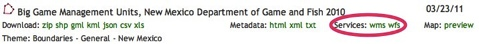
\includegraphics{images/RGIS_OGCLinkScreenshot.jpg}
\caption{Illustration highlighting where to see if a spacific dataset
has an available OGC service}
\end{figure}

\emph{Important}: When adding any WFS layer, you may need to go into the
preferences for QGIS and under the ``Network'' options increase the
``Timeout for Network Requests(ms)'' value to a larger number than the
default 60000 (1 minute). If you don't do this, QGIS might give up on
the request before it has been fulfilled by the server. You may also
want to zoom into a limited area and check the box in the QGIS ``Add WFS
Layer \ldots{}'' dialog for ``Only Request Features Overlapping the
Current View Extent'' as this will reduce the number of features
recovered - a significant issue if the WFS service is publishing a large
number of features.

In your write-up include the names of the layers you added, and the
GetCapabilities requests related to those layers. Also include screen
shots (again, one for each added layer) showing each layer in your QGIS
project. 


\chapter{Week 13 - Platforms and GeoServer Introduction}\label{week13}

Thus far we have concentrated on the client side of geospatial services
oriented architectures in developing web interfaces based upon the
Google Maps API, the OpenLayers javascript framework, and accessing data
published using the OGC WMS, WFS, and WCS standards in desktop
applications. Starting this week we begin our work on the server side -
working with the GeoServer server platform to publish data through the
OGC WMS, WFS, and WCS service standards. This work will demonstrate the
ease with which you can share data using these standards, facilitating
client use such as that that we have seen in our web site and desktop
application work.

\emph{Expected Outcomes}

By the end of this class, students should be able to:

\begin{itemize}
\tightlist
\item
  Place files within the server file system for integration into the
  GeoServer platform
\item
  Create a GeoServer \emph{Workspace}, \emph{Store}, and \emph{Layer}
  based upon those data
\item
  Test those layers using the \emph{Layer Preview} tools integrated into
  GeoServer
\end{itemize}

\emph{Key Concepts}

By the end of this class, students should understand:

\begin{itemize}
\tightlist
\item
  The components of a map server platform and their relationship to each
  other
\item
  The role of a geospatial server within a geospatial services oriented
  architecture
\item
  The information required about data to successfully configure it for
  publication within GeoServer
\item
  The stepwise process through which a dataset may be published using
  GeoServer
\end{itemize}

\section{Reference Materials}\label{week13-reference}

\begin{itemize}
\tightlist
\item
  Lynda.com
  \href{http://www.lynda.com/Linux-tutorials/Learn-Linux-Command-Line-Basics/435539-2.html?org=unm.edu}{\emph{Learn
  the Linux Command Line: The Basics}} - particularly:

  \begin{itemize}
  \item
    Introduction
  \item
    \begin{enumerate}
    \def\labelenumi{\arabic{enumi}.}
    \tightlist
    \item
      Command-Line Basics
    \end{enumerate}
  \item
    \begin{enumerate}
    \def\labelenumi{\arabic{enumi}.}
    \setcounter{enumi}{1}
    \tightlist
    \item
      Files, Folders, and Permissions
    \end{enumerate}
  \end{itemize}
\item
  GeoServer
  \href{http://docs.geoserver.org/stable/en/user/index.html}{Online
  Documentation}: sections
  \href{http://docs.geoserver.org/stable/en/user/introduction/index.html}{Introduction},
  \href{http://docs.geoserver.org/stable/en/user/gettingstarted/index.html}{Getting
  Started}, and
  \href{http://docs.geoserver.org/stable/en/user/webadmin/index.html}{Web
  Administration Interface}
\end{itemize}

\section{Weekly Milestone - Linux Basics and GeoServer Data
Import}\label{week13-milestone}

\subsection{Working on the Class
Server}\label{working-on-the-class-server}

For the GeoServer portion of our work, you will be working on a Linux
server that has been created for the class. While we won't be doing a
lot of Linux work, some basic familiarity with moving around, copying
files, and working with files is needed. The class server is running
Ubuntu Linux which is a broadly deployed, well supported operating
system and computing platform that has excellent support for many Open
Source geospatial applications, including those that we will be using in
this class.

The first set of exercises relate to learning some basics about working
with the Linux Operating system, applicable just about any Linux server
including the class server.

Review (but don't worry about memorizing) the following materials (in
addition to watching the Lynda.com video tutorial sections listed
above):

\href{http://www.webmonkey.com/2010/02/unix-guide/}{Webmonkey ``Unix
Guide''}

\href{http://www.cheatography.com/davechild/cheat-sheets/linux-command-line/}{Linux
Command Line Cheatsheet}

\begin{description}
\tightlist
\item[QUESTION 1]
What command would you use to list the contents of a directory on a
linux system?
\item[QUESTION 2]
What command would you use to read the ``manual page'' for a specific
command?
\end{description}

Log into the class Linux server - geog485.unm.edu. \emph{This is
different from the address referenced in the below linked videos} The
rest of the process is the same as demonstrated in the videos.

\emph{Windows}: Open PuTTY on your computer and connect using the SSH
protocol (see video demonstration)

\href{http://youtu.be/GdO_n89mey8}{Link to the YouTube video
demonstration for Windows}

\emph{Mac}: Open the Terminal Application and connect using SSH (see
video)

\href{http://youtu.be/Gu_ij6HxTWo}{Link to the YouTube video
demonstration for Mac OS X}

Start a session on the class Linux server, which is located at at the
hostname \texttt{geog485.unm.edu} (you will use your class server
username and password to open the connection)

\begin{description}
\tightlist
\item[Task]
Use the \texttt{mkdir\ data} command to create a directory called
\texttt{data} in your home directory (the directory that you are in when
you login, and where you go when you type the \texttt{cd} command with
no options).
\end{description}

\subsection{Adding data to GeoServer}\label{adding-data-to-geoserver}

To add data to GeoServer you must have a file location on the server
where data files must be stored and accessible by the GeoServer.

\begin{description}
\item[Task]
Change into the \texttt{data} directory that you created above using the
\texttt{cd\ data} command.
\item[Task]
Copy all of the data files located in the \texttt{data} directory in my
\texttt{Week13Data} folder by executing the following command from
\emph{inside your \texttt{data} directory}.

cp -r /geodata/data/demo/week13data/* . (make sure to include final `.')
\end{description}

This will place a copy of these data files in your \texttt{data}
directory

\begin{description}
\tightlist
\item[Task]
Log into the Geoserver on the class server
(\url{http://geog485.unm.edu:8080/geoserver/web/}) using the username
and password provided for the class server via email.
\end{description}

Create a new \emph{store} for each of the datasets added to your
\texttt{data} directory above. Assign the new store to the workspace
that is named based on your username (e.g.
\texttt{ws\_\textless{}your\ user\ name\textgreater{}}. When specifying
the the \texttt{Connection\ Parameters} for pointing to the file, the
format is:
\texttt{file:data/\textless{}your\ username\textgreater{}/data/\textless{}filename\ including\ any\ additional\ directories\textgreater{}}

for example

\begin{verbatim}
file:data/kbene/data/roadl_usa.shp
\end{verbatim}

You can also browse to the file by clicking on the ``Browse \ldots{}''
link next to the location field, for example for a shapefile:

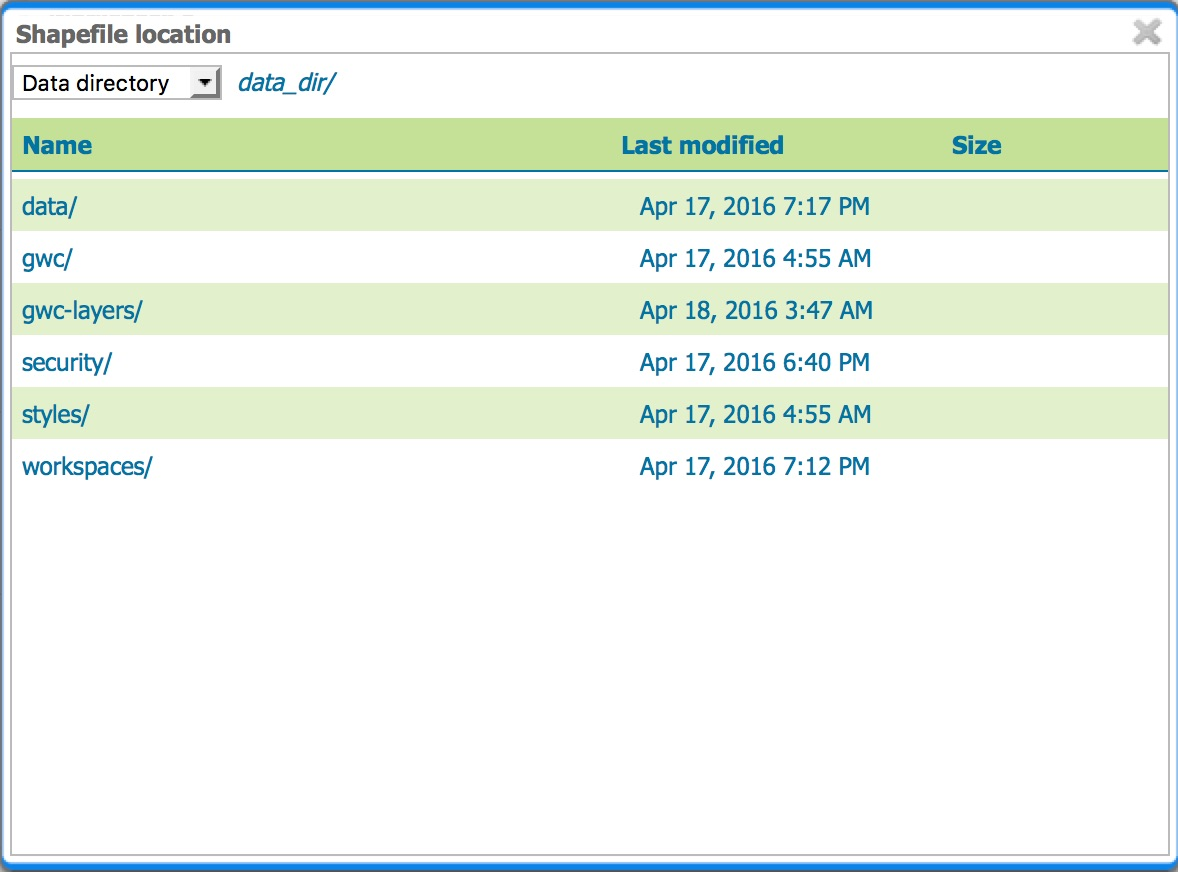
\includegraphics{images/GeoServer_Browse.jpg}~

and navigating to your home directory (data\_dir/data/\textless{}your
username\textgreater{}/data) to see the data to select from.

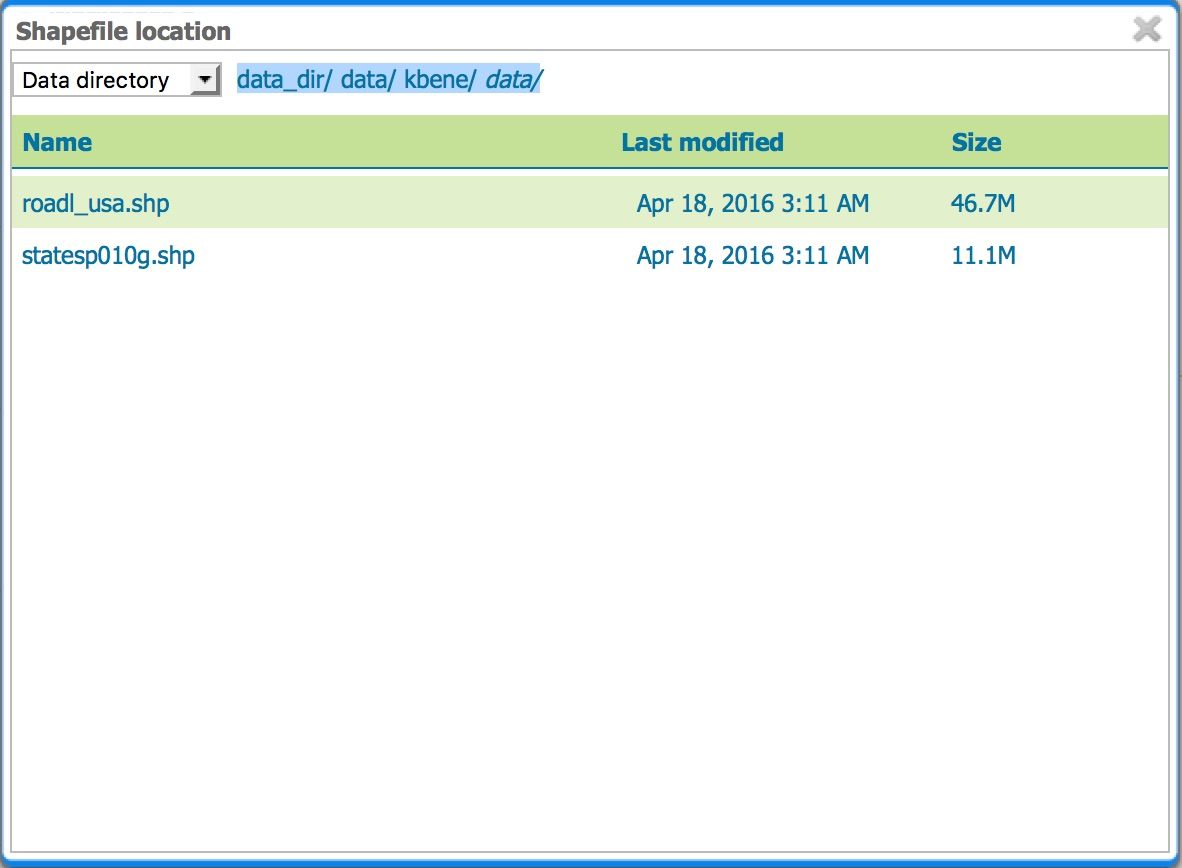
\includegraphics{images/GeoServer_SelectData.jpg}~

Create a new \emph{layer} for each of the \emph{stores} added above.
Here are some things to keep in mind:

You may need to designate the SRS for a layer if it can't be read
directly from the dataset. Your specify the \emph{designated} SRS using
the standard EPSG:XXXX format.

The EPSG code for \texttt{GCS\_North\_American\_1983} is EPSG:4269

\begin{description}
\tightlist
\item[Question 3]
Preview each of your added layers, using the \emph{Layer Preview} tool
and the \emph{Open Layers} option to display the data. Include screen
grabs of the previews in your write-up.
\end{description}

\chapter{Week 14 - OGC Services and Styling in GeoServer}\label{week14}

While integrating data into a web mapping platform is a critical first
step, a robust geospatial data service system must also support the
development and use of cartographically informative representations of
the published data. GeoServer accomplishes this through the integration
of the Open Geospatial Consortium's Styled Layer Descriptor standard
into the system for publishing alternative styles for vector and raster
data products. This standard allows for the configuration of attribute
and scale-based representations that may be advertised by name and
requested by reference through the published OGC WMS services.

\emph{Expected Outcomes}

At the end of this class students will be able to:

\begin{itemize}
\tightlist
\item
  Develop a basic SLD for a vector layer within GeoServer
\item
  Define an attribute filter as part of an SLD to allow for differential
  representation of features based upon the values of one or more
  attribute values
\item
  Define a scale limit filter as part of an SLD to control the scales at
  which a defined SLD rule will be executed
\end{itemize}

\emph{Key Concepts}

At the end of this class, students will understand:

\begin{itemize}
\tightlist
\item
  The role of the OGC SLD standard in defining and publishing geospatial
  data via WMS
\item
  The capabilities of the SLD standard to defined representation styles
  that may be defined in reference to attribute values and WMS request
  scales
\item
  That logical comparison operators may be used to control the
  application of style rules to specific features
\end{itemize}

\section{Reference Materials}\label{week14-reference}

\begin{itemize}
\tightlist
\item
  GeoServer
  \href{http://docs.geoserver.org/stable/en/user/index.html}{Online
  Documentation}: sections
  \href{http://docs.geoserver.org/latest/en/user/data/index.html\#data}{Data
  Management},
  \href{http://docs.geoserver.org/latest/en/user/styling/index.html\#styling}{Styling}
\end{itemize}

\section{Weekly Milestone - Styling of Layers in
GeoServer}\label{weekly-milestone---styling-of-layers-in-geoserver}

This week's milestone provides an opportunity to experiment with vector
layer styling. Please define two custom styles for each of the vector
datasets that you added to GeoServer during last week's lab assignment.
Take a screenshot of the layer preview for each of your styles -
including the options tools above the OpenLayers preview displaying the
name of the custom style that is being used for the current map display.

Include in your writeup the layer name, the name of the two custom
styles and the associated screenshots for each of the vector datasets.

\section{Deep Dive - Data Integration and Styling in
GeoServer}\label{deep-dive---data-integration-and-styling-in-geoserver}

Add each of the datasets that you acquired for Deep Dive 3 to GeoServer
and style at least three of the layers with a custom style designed to
best display the data for your envisioned map. Include in your writeup
the names of the datasets, associated styles, and screenshots of the
layers in the OpenLayers previewer, with the style name displayed in the
OpenLayers preview tool set.

\chapter{Week 15 - OGC Services and Styling in GeoServer}\label{week15}

Thus far we have discussed the general workflow for publishing
geospatial data using GeoServer, the general concepts relating to
styling those data for presentation through the web services published
by GeoServer, and specific methods for styling vector data, and applying
styles to specific subsets of vector data through the use of filters.
This week we conclude our discussion of GeoServer with a demonstration
of the methods used in the styling of raster data. Without the
application of meaningful styles, raster data can be visually
unintelligible. You will learn the tools that you have within the OGC
Styled Layer Descriptor standard (as implemented within GeoServer) to
define and apply meaningful styles to raster data - ultimately producing
more useful visualizations of those data.

\emph{Expected Outcomes}

At the end of the class, students will be able to:

\begin{itemize}
\tightlist
\item
  Define ColorMaps for raster data that produce a continuous gradient of
  colors, a stepped color ramp between defined raster values, and color
  assignments for specific raster values.
\item
  Map bands from a multi-band raster file to the RGB colors used to
  generate a color map image or to a single grayscale band for
  generating a single-band representation.
\item
  Define opacity for an entire raster dataset or on a per-value level
  within a ColorMap.
\item
  Apply a variety of contrast enhancements to individual color bands to
  improve/modify the display of the overall map image.
\end{itemize}

\emph{Key Concepts}

At the end of the class, students will understand:

\begin{itemize}
\tightlist
\item
  The concepts of continuous color ramps, color intervals, and colors
  assigned to individual raster values as alternative representation
  models for raster data
\item
  The concept of a multi-band raster image and the mapping of specific
  raster bands into the RGB color space for visual representation
\item
  Two methods for defining opacity for a raster dataset as a whole or
  for individual values
\item
  The options for and potential effects of contrast enhancement on
  raster map images.
\end{itemize}

\section{Reference Materials}\label{week15-reference}

\begin{itemize}
\tightlist
\item
  GeoServer
  \href{http://docs.geoserver.org/stable/en/user/index.html}{Online
  Documentation}: sections
  \href{http://docs.geoserver.org/latest/en/user/data/index.html\#data}{Data
  Management},
  \href{http://docs.geoserver.org/latest/en/user/styling/index.html\#styling}{Styling}
\end{itemize}

\section{Weekly Milestone - Create a Final OpenLayers
Client}\label{weekly-milestone---create-a-final-openlayers-client}

Please create a final OpenLayers mapping client that displays the
GerServer-based Styled WMS layers that you created for Deep Dives 3 \&
4, focusing on the goals that were laid out in Deep Dive 3. Include in
your mapping client a narrative description (a paragraph or two, aimed
at a novice user coming to your page for the first time) of the goals
and data contained within the client.

\section{Peer Review -}\label{week15-peerReview}

\emph{Peer Review:} This week's assignment will include a peer review
component. Specifically, 1/3 of your 20-point peer review score will be
based upon \emph{your} peer-review of \emph{two} other web pages
generated by the students in the class. The required peer-review will
consist of two steps:

\begin{enumerate}
\def\labelenumi{\arabic{enumi}.}
\item
  Create a new Discussion Thread in Learn entitled: ``Page for
  Peer-Review \textless{}Your Name\textgreater{}'' at the same time you
  link your milestone to your homepage. Include in the post the GitHub
  address of your Week 10 milestone that you created for this
  assignment.
\item
  Provide a \emph{substantive}, \emph{constructive}, and \emph{civil}
  comment (through the ``reply'' option for a posted thread) to
  \emph{two} of the posted discussion threads posted for peer-review.
  Please complete the peer-review as soon as possible so that your
  colleagues can benefit most from your input. Complete the peer-review
  no later than the required end-of-term portfolio review deadline.
  Think about the following ideas for your review: \emph{what did I
  learn from this page}, \emph{what was done well}, \emph{what could be
  improved}
\end{enumerate}

\begin{center}\rule{0.5\linewidth}{\linethickness}\end{center}

This work by {Karl Benedict} is licensed under a Creative Commons
Attribution-ShareAlike 4.0 International License.

\end{document}
